\documentclass[a4paper,titlepage]{report}

\usepackage{booktabs} 
\usepackage{adjustbox} 

% Packages for graphics and layout
\usepackage{graphicx}
\usepackage[a4paper, margin=1in]{geometry}
\usepackage{titlesec}
\usepackage[dvipsnames]{xcolor}
\usepackage{colortbl}
\usepackage{caption}
\usepackage{calc}
\usepackage{ragged2e}
\usepackage{mdframed}
\usepackage{tikz}
\usepackage{svg}

\usepackage{subcaption} % add this for subfigure support


% Packages for math and tables
\usepackage{amsmath}
\usepackage{booktabs}
\usepackage{cellspace} % For adding padding in table cells
\usepackage{tabularx}
\usepackage{multirow}
\usepackage{array}
\usepackage{longtable}

% Packages for references and the table of contents
\usepackage{hyperref} % For links in the table of contents
\usepackage{tocbibind} % To include the table of contents in the table of contents

% Packages for code
\usepackage{listings}
\usepackage{courier} % Font for code
\usepackage{fancyvrb}
\usepackage{lipsum} % For dummy text

% Remove paragraph indentation and add space between paragraphs
\usepackage{parskip}  
\usepackage{algorithm}
\usepackage{algpseudocode}

\algdef{SE}% flags used internally to indicate we're defining a new block statement
[CLASS]% new block type, not to be confused with loops or if-statements
{Class}% "\Struct{name}" will indicate the start of the struct declaration
{EndClass}% "\EndStruct" ends the block indent
[1]% There is one argument, which is the name of the data structure
{\textbf{class} \textsc{#1}}% typesetting of the start of a struct
{\textbf{end class}}% typesetting the end of the struct


\algdef{SE}% flags used internally to indicate we're defining a new block statement
[METHOD]% new block type, not to be confused with loops or if-statements
{Method}% "\Struct{name}" will indicate the start of the struct declaration
{EndMethod}% "\EndStruct" ends the block indent
[2]% There is one argument, which is the name of the data structure
{\textbf{method} \textsc{#1}(\textsc{#2})}% typesetting of the start of a struct
{\textbf{end method}}% typesetting the end of the struct


\usepackage[utf8]{inputenc} % To handle UTF-8 encoding
\usepackage[T1]{fontenc}    % To ensure proper font encoding
\usepackage{lmodern}        % Latin Modern font which supports Turkish characters
\usepackage[english]{babel}
\usepackage{algorithmicx}


% Set the table format for the combiner and in mapper part
\setlength{\extrarowheight}{5pt} % Extra vertical padding
\setlength{\tabcolsep}{10pt} % Extra horizontal padding

% Define custom colors
\definecolor{myBlue}{rgb}{0.0745, 0.2157, 0.4118}
\definecolor{myLightBlue}{rgb}{0, 0.5647, 0.5843}
\definecolor{myGray}{RGB}{192,197,206}
\definecolor{myPurple}{rgb}{0.5, 0.0, 0.5} % Esempio di colore viola
\definecolor{myLightPurple}{HTML}{CC0066} % Esempio di colore viola chiaro
\definecolor{jsonString}{HTML}{111258}
\definecolor{numb}{RGB}{255,0,0}
\definecolor{punct}{RGB}{0,0,255}
\definecolor{delim}{RGB}{20,105,176}
\definecolor{comment}{RGB}{0,128,0}
\definecolor{string}{RGB}{163,21,21}
\definecolor{keyword}{RGB}{0,0,255}
\definecolor{darkgreen}{rgb}{0,0.5,0}
\definecolor{java_keyword}{HTML}{BF9B30}
\definecolor{java_comment}{HTML}{0000FF}
\definecolor{mybackgroundcolor}{RGB}{240, 240, 240} % Light gray background
\definecolor{black}{RGB}{0, 0, 0} % Define black color
\definecolor{jsondoc}{HTML}{C4E3E8}
\definecolor{red}{HTML}{8F1D39}
\definecolor{white}{RGB}{255,255,255} % Define white color



% Configuration for hyperref to remove red margins and color the links
\hypersetup{
    colorlinks=true,
    linkcolor=black,
    filecolor=magenta,
    urlcolor=myPurple,
    linkbordercolor={0 0 0} % Set link border color to black (invisible)
}

% Configuration for section titles
\titleformat{\section}[hang]{\Large\bfseries\color{myPurple}}{}{0px}{}[\titlerule]
\titleformat{\subsection}[hang]{\large\bfseries\color{myLightPurple}}{}{0em}{}
\titleformat{\subsubsection}[hang]{\bfseries\color{myPurple}}{}{0em}{}

% Configuration for chapter titles
\titleformat{\chapter}[display]
  {\normalfont\Large\bfseries\color{myPurple}}{}{-80pt}{\LARGE}
\renewcommand{\chaptername}{} % Remove the word "Chapter" and the number from the title
\setcounter{tocdepth}{1} % Include only chapters and sections in the table of contents

% Style for code
\lstdefinestyle{mystyle}{
    language=Java,
    backgroundcolor=\color{mybackgroundcolor}, % Background color
    commentstyle=\color{darkgreen},
    keywordstyle=\color{blue},
    numberstyle=\tiny\color{gray},
    stringstyle=\color{orange},
    basicstyle=\ttfamily\footnotesize,
    framesep=10pt, % padding between frame and text
    xleftmargin=10pt, % left margin
    xrightmargin=10pt, % right margin
    aboveskip=10pt, % Top padding
    belowskip=10pt, % Bottom padding
    breakatwhitespace=false,         
    breaklines=true,                 
    captionpos=b,                    
    keepspaces=true,                 
    numbers=left,                    
    numbersep=5pt,                  
    showspaces=false,                
    showstringspaces=false,
    showtabs=false,                  
    tabsize=2
}

% Define a custom style for mdframed
\mdfdefinestyle{customstyle}{
    linecolor=myBlue, % Border color
    linewidth=2pt, % Border width
    roundcorner=10pt, % Rounded corners
    backgroundcolor=mybackgroundcolor, % Background color
    innertopmargin=10pt, % Top padding
    innerbottommargin=10pt, % Bottom padding
    innerrightmargin=10pt, % Right padding
    innerleftmargin=10pt, % Left padding
    skipabove=20pt, % Space above the frame
    skipbelow=20pt, % Space below the frame
    fontcolor=black, % Text color
}

% Define a custom style for mdframed
\mdfdefinestyle{customstyle2}{
    linecolor=myBlue, % Border color
    linewidth=2pt, % Border width
    roundcorner=10pt, % Rounded corners
    backgroundcolor=white, % Background color
    innertopmargin=10pt, % Top padding
    innerbottommargin=10pt, % Bottom padding
    innerrightmargin=10pt, % Right padding
    innerleftmargin=10pt, % Left padding
    skipabove=20pt, % Space above the frame
    skipbelow=20pt, % Space below the frame
    fontcolor=black, % Text color
}





\begin{document}

\begin{titlepage}
    \centering
    \vspace*{\fill}
    {\LARGE \textbf{UNIVERSITY OF PISA}}\\[0.5cm]
    \begin{figure}[h]
        \centering
        
\includegraphics[width=0.4\textwidth]{media/university-of-Pisa-logo.jpg}
    \end{figure}
    {\Large \textit{Artificial Intelligence and Data Engineering}}\\[1.5cm]
    {\LARGE \textbf{Data Mining and Machine Learning}}\\[1cm]
    {\Large \textit{Music popularity across borders}}\\[2cm]
    
    {\large \textbf{Noemi Cherchi, Feyzan Çolak}}\\[0.5cm]
    {\large Academic Year 2023/2024}
    \vspace*{\fill}
\end{titlepage}

\tableofcontents

\chapter{Introduction}

The music industry plays a significant role in today’s globalized world as it has been growing rapidly over the years. It also faces the unique challenge of addressing diverse audiences across
different countries. Each country has different tastes in music which are shaped
by lots of factors. For a record label, it is crucial to understand these preferences for a successful music promotion and marketing. The ability to predict
the popularity of a song before it is released can provide a significant 
competitive privilege.\\
\\
This project aims to analyze the varying musical preferences across different countries by 
exploring their popular songs and understanding what makes those songs popular. In particular, specific audio features have been taken in consideration,  
such as danceability, key, loudness, mode, speechiness and acousticness. 
By leveraging Data Mining and Machine Learning Techniques, this project will provide insights into
the factors determining the popularity of songs in different countries.\\


\section{Dataset}
The final dataset used in this project is obtained by combining two different and extensive datasets.

The first dataset was taken from the following Kaggle \href{https://www.kaggle.com/datasets/dhruvildave/spotify-charts/data} {link}. \\

This dataset is called Spotify Charts and contains information about the most popular songs in different countries. It is a complete dataset 
of all the "Top 200" and "Viral 50" charts published globally by Spotify. Spotify publishes a new chart
 every 2-3 days. This is Spotify's entire collection since January 1, 2017.
 The included key details are the song's name, artist, spotify id, rank, and the number of streams 
 in each country. This dataset is helpful to undertand how musical preferences change across different
 parts of the world. \\

 The second dataset was created by individuating all the unique song IDs from the first dataset and using the Spotify API to gather the audio features of more than 200K songs. The audio features that are used in this project are $danceability, energy, key, loudness, mode, speechiness, acousticness$, 
 $instrumentalness, liveness, valence, tempo, duration (ms), time signature$.  
 These features are essential for analyzing the musical elements that contribute to a song's popularity in each country.\\

 Before starting the preprocessing phase, the two datasets were merged togethere by the Spotify ID. This ensured that the audio features from the Spotify API were 
 correctly associated with the corresponding songs and their popularity metrics in different countries.\\


\newpage
 \section{Audio Features}

 \begin{table}[ht]
    \centering
    \resizebox{\textwidth}{!}{ % Resize table to fit within text width
    \begin{tabular}{|>{\raggedright\arraybackslash}p{0.15\textwidth}|>{\raggedright\arraybackslash}p{0.12\textwidth}|>{\raggedright\arraybackslash}p{0.73\textwidth}|}
    \hline
    \textbf{Feature} & \textbf{Data Type} & \textbf{Description} \\
    \hline
    Danceability & float & Describes how suitable a track is for dancing based on a combination of musical elements. A value of 0.0 is least danceable and 1.0 is most danceable. \\
    \hline
    Energy & float & Measure from 0.0 to 1.0 and represents a perceptual measure of intensity and activity. Typically, energetic tracks feel fast, loud, and noisy. For example, death metal has high energy, while a Bach prelude scores low on the scale. \\
    \hline
    Key & integer & The key the track is in. Integers map to pitches using standard Pitch Class notation. If no key was detected, the value is -1. \\
    \hline
    Loudness & float & The overall loudness of a track in decibels (dB). Loudness values are averaged across the entire track and are useful for comparing relative loudness of tracks. It is the quality of a sound that is the primary psychological correlate of physical strength (amplitude). Values typically range between -60 and 0 dB. \\
    \hline
    Mode & integer & Mode indicates the modality (major or minor) of a track, the type of scale from which its melodic content is derived. Major is represented by 1 and minor is 0. \\
    \hline
    Speechiness & float & Speechiness detects the presence of spoken words in a track. Speech-like the recording (e.g. audio book, poetry), the closer to 1.0 the attribute value. Values above 0.66 describe tracks that are probably made entirely of spoken words. Values between 0.33 and 0.66 describe tracks that may contain both music and speech, either in sections or layered, including such cases as rap music. Values below 0.33 most likely represent music and other non-speech-like tracks. \\
    \hline
    Acousticness & float & A confidence measure from 0.0 to 1.0 of whether the track is acoustic. 1.0 represents high confidence the track is acoustic. \\
    \hline
    Instrumentalness & float & Predicts whether a track contains no vocals. "Ooh" and "aah" sounds are treated as instrumental in this context. The closer the instrumentalness value is to 1.0, the greater likelihood the track contains no vocal content. Values above 0.5 are intended to represent instrumental tracks, but confidence is higher as the value approaches 1.0. \\
    \hline
    Liveness & float & Detects the presence of an audience in the recording. Higher liveness values represent an increased probability that the track was performed live. A value above 0.8 provides strong likelihood that the track is live. \\
    \hline
    Valence & float & A measure from 0.0 to 1.0 describing the musical positiveness conveyed by a track. Tracks with high valence sound more positive, while tracks with low valence sound more negative. \\
    \hline
    Tempo & float & The overall estimated tempo of a track in beats per minute (BPM). In musical terminology, tempo is the speed or pace of a given piece and derives directly from the average beat duration. \\
    \hline
    Duration (ms) & integer & The duration of the track in milliseconds. \\
    \hline
    Time Signature & integer & An estimated time signature. The time signature (meter) is a notational convention to specify how many beats are in each bar (or measure). The time signature ranges from 3 to 7 indicating time signatures of "3/4", to "7/4". \\
    \hline  
    \end{tabular}
    }
\end{table}
\chapter{Data Preprocessing}
\chapter{Data Visualization}

The final dataset has 189297 rows × 15 columns. The columns are as follows: 
\begin{table}[h!]
    \centering
    \begin{tabular}{lllll} % 5 columns per row
    \toprule
    \textbf{danceability} & \textbf{energy} & \textbf{key} & \textbf{loudness} & \textbf{mode} \\
    \textbf{speechiness} & \textbf{acousticness} & \textbf{instrumentalness} & \textbf{liveness} & \textbf{valence} \\
    \textbf{tempo} & \textbf{duration\_ms} & \textbf{time\_signature} & \textbf{region} & \textbf{popular} \\
    \bottomrule
    \end{tabular}
    \caption{Column names in the dataset}
\end{table}

By visualizing and exploring the final dataset, we can underline the differeces with the raw dataset. This shows that the preprocessing phase was fundamental to obtain a clean dataset.

\begin{verbatim}
    # Display the first few rows of the dataset
    df.head()
    
    # Display basic information about the dataset
    df.info()
    \end{verbatim}
    
    \begin{figure}[h]
        \centering
        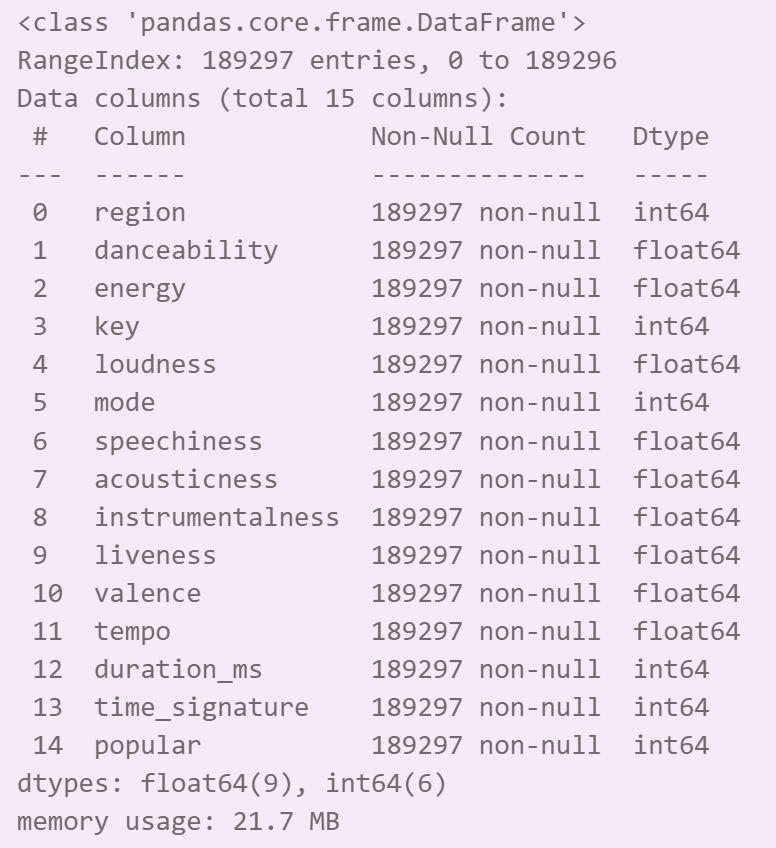
\includegraphics[width=0.5\textwidth]{media/info_cleaned.png} 
        \caption{Basic information.}
        \label{df.info()}
    \end{figure}

    One of the first thing to notice is how the memory usage has been reduced significantly. This is due to the removal of columns that were not useful for the analysis. In fact, the number of columns has been reduced from 26 to 15.
    
    \newpage
    \begin{verbatim}
    # Summary statistics of the dataset
    df.describe()
    \end{verbatim}
    
    
    \begin{figure}[h]
        \centering
        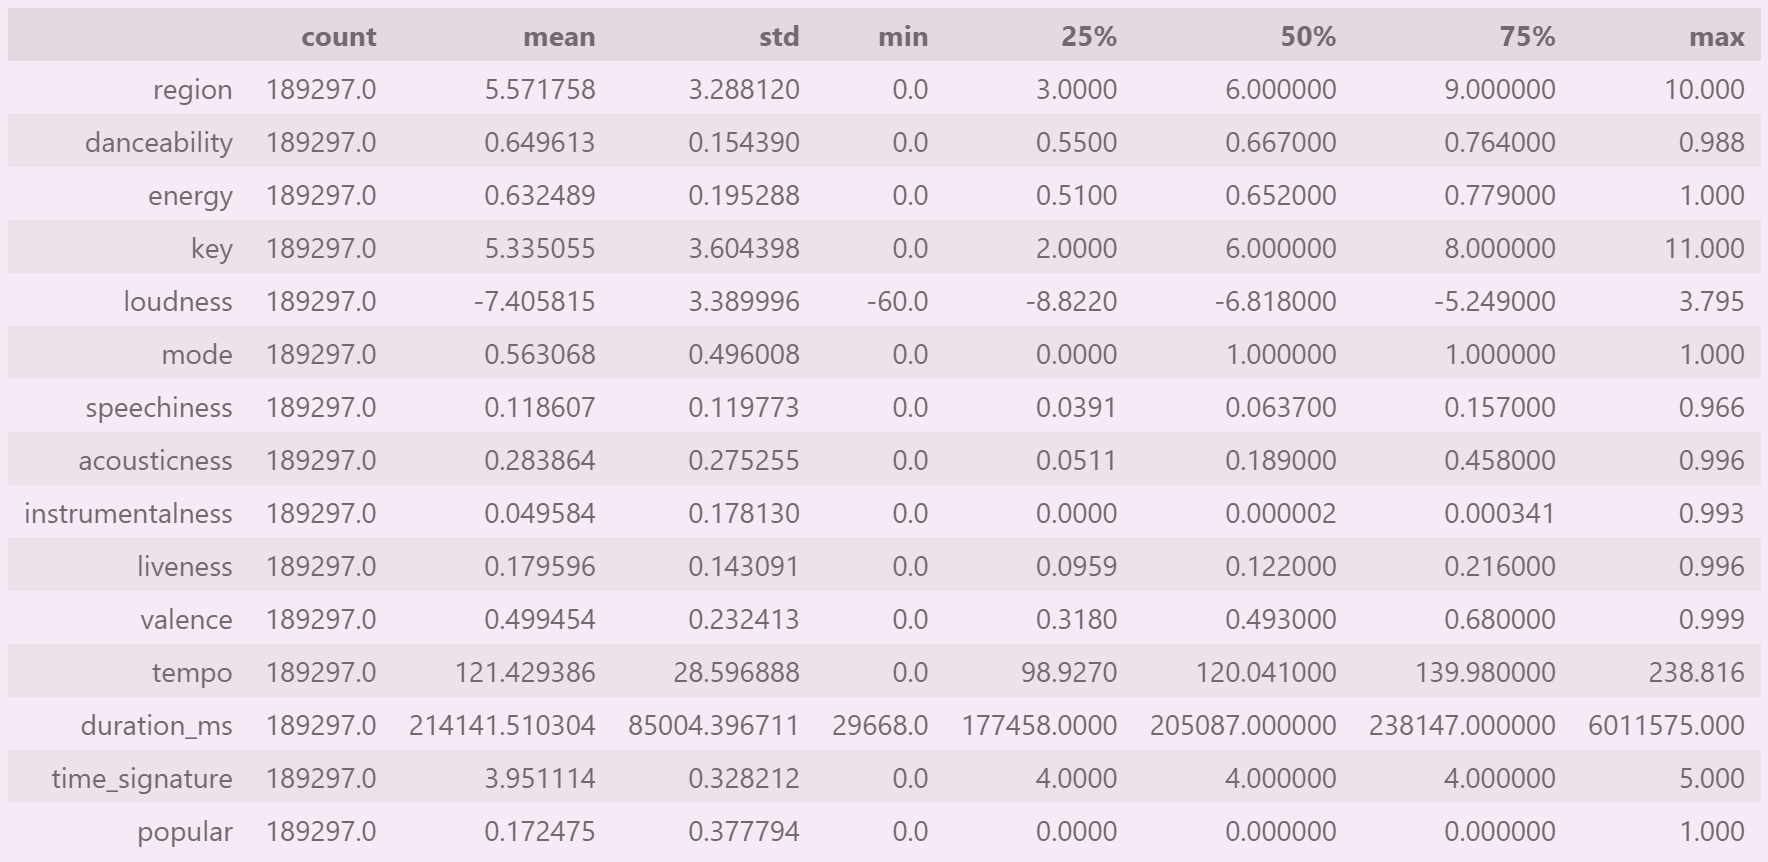
\includegraphics[width=1.1\textwidth]{media/describe_cleaned.png} 
        \caption{Summary statistics of the dataset.}
        \label{df.describe()}
    \end{figure}

The popular songs represent about the 20\% of the dataset.

    \begin{figure}[h]
        \centering
        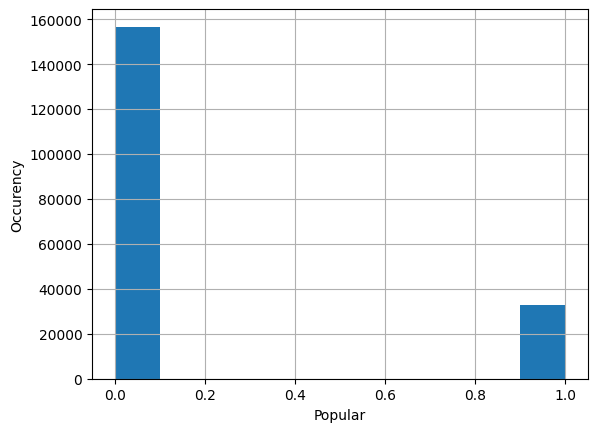
\includegraphics[width=0.5\textwidth]{media/popular_dist_cleaned.png} 
        \caption{Distribution of popular songs.}
        \label{popular_songs}
    \end{figure}

\newpage

Each audio feature is distributed in this way: 

\begin{figure}[h]
    \centering
    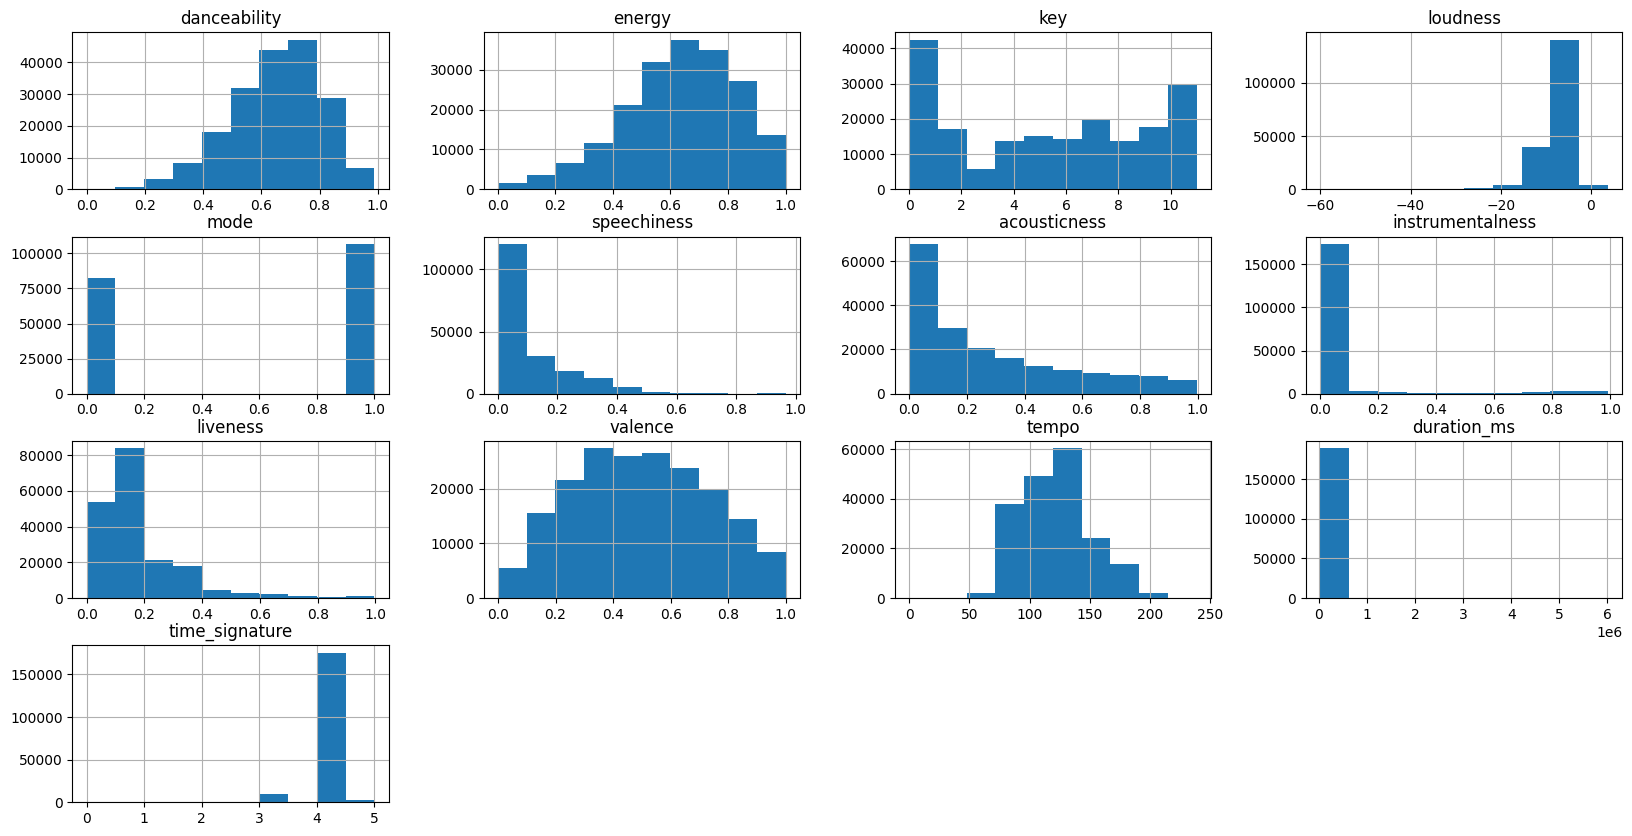
\includegraphics[width=0.9\textwidth]{media/feature_dist_cleaned.png} 
    \caption{Distribution of audio features.}
    \label{distribution}
\end{figure}

This is the boxplot of the audio features:

\begin{figure}[h]
    \centering
    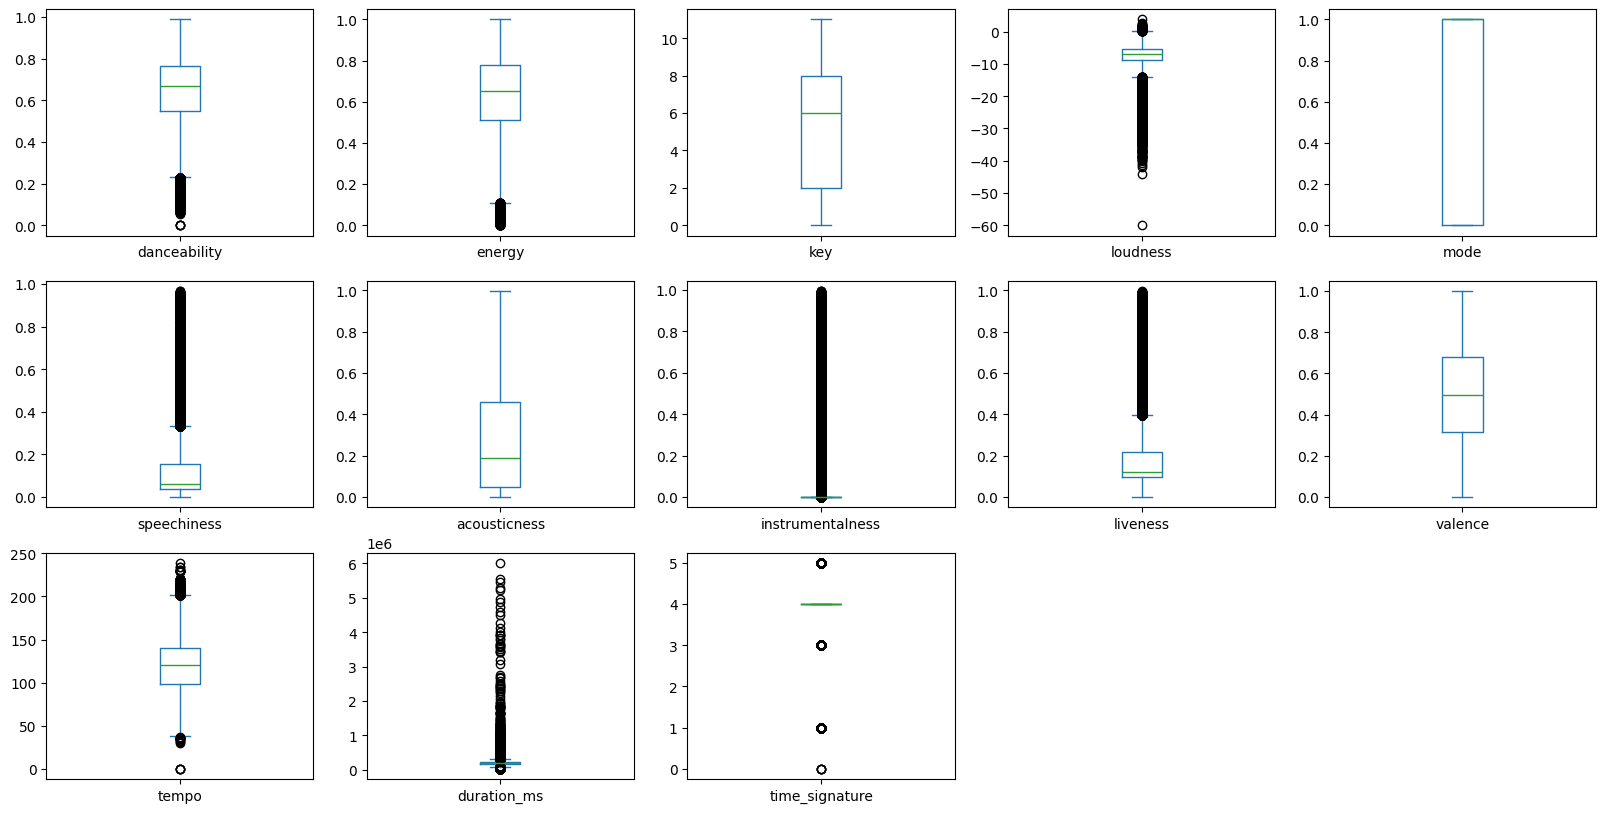
\includegraphics[width=0.9\textwidth]{media/boxplot_cleaned.png} 
    \caption{Boxplot of audio features.}
    \label{boxplot}
\end{figure}


Many features have outliers (especially loudness, instrumentalness, speechiness, and duration\_ms), which means they have songs that are very different from the "average" in terms of these attributes.
Features like mode and time\_signature have almost no variation, thus they may not be useful for predicting the target variable (popularity).


\newpage

This is the heatmap of the correlation matrix:

\begin{figure}[h]
    \centering
    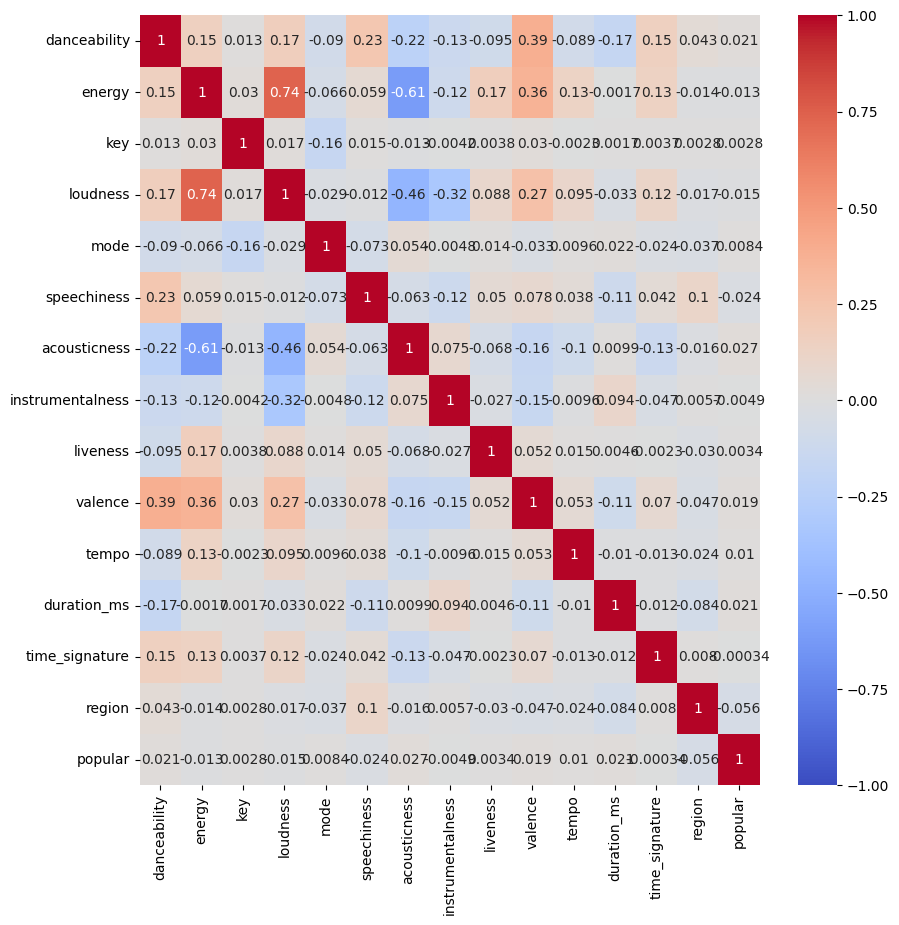
\includegraphics[width=0.9\textwidth]{media/heatmap_cleaned.png} 
    \caption{Heatmap of the correlation matrix.}
    \label{correlation}
\end{figure}

The heatmap shows that the audio features have a mix of positive and negative correlations with each other. The most notable correlations are:
\begin{itemize}
    \item 
    Energy and Loudness: strong positive correlation (0.74). Loud songs tend to also have high energy, which makes sense musically.
    \item Energy and Acousticness: strong negative correlation  (-0.61). Acoustic songs tend to have lower energy levels, which aligns with expectations as acoustic songs are often more mellow.
\end{itemize}


This also shows us that no single feature stands out as highly predictive of song popularity based on these correlations, which suggests that popularity might be determined by a complex interaction of features rather than individual attributes. 



\newpage

We can also visualize the popularity of each feature in the different regions:

\begin{figure}[h]
    \centering
    \begin{minipage}{0.45\textwidth}
        \centering
        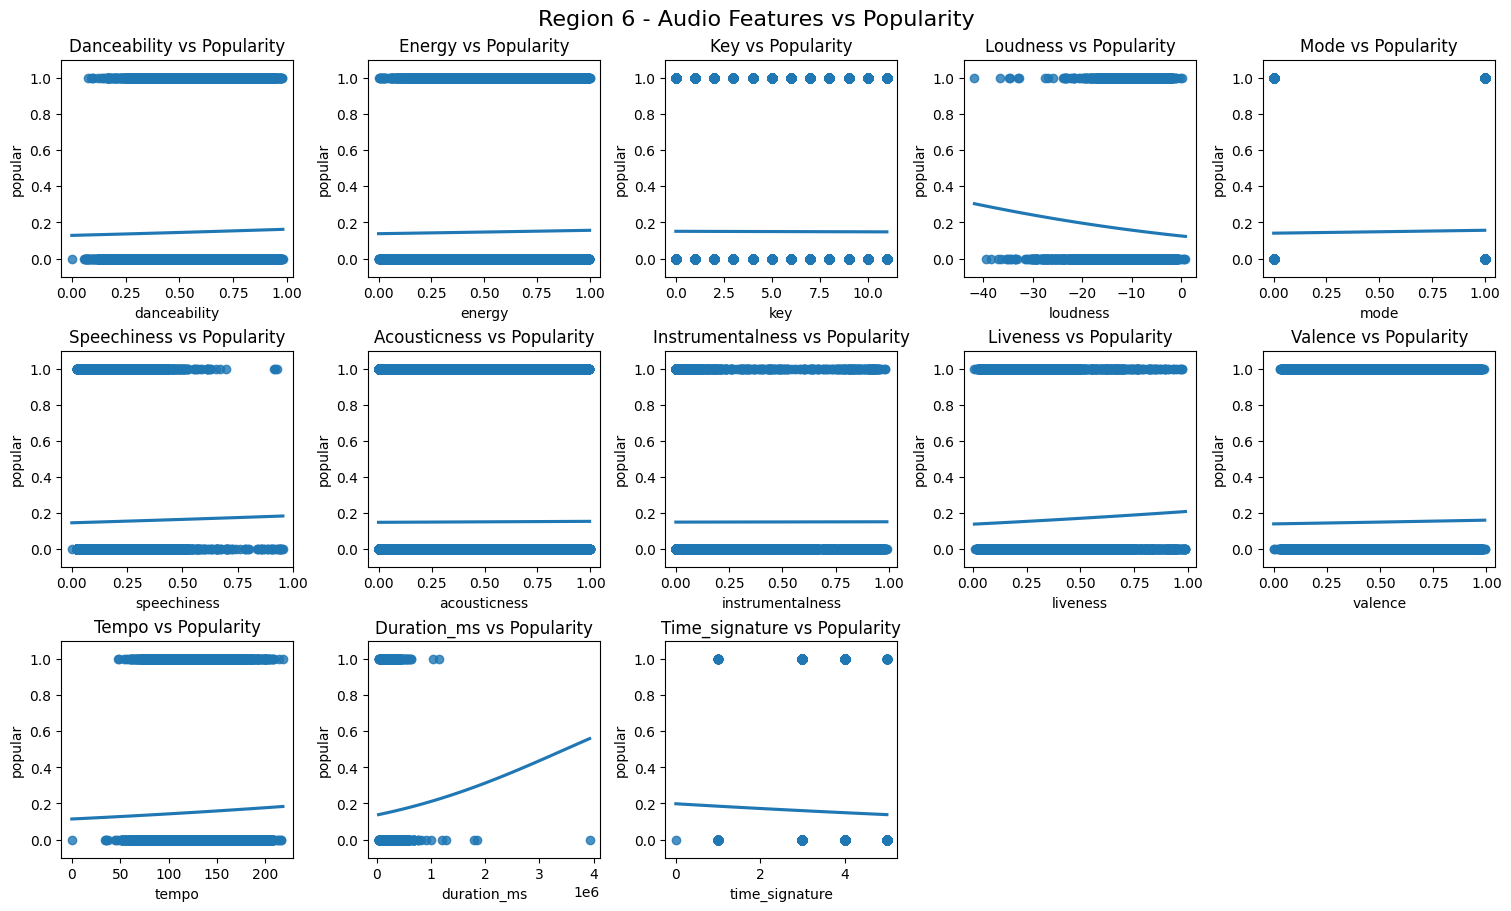
\includegraphics[width=\linewidth]{media/region6_cleaned.png}
        \caption{Popularity in Northern Europe}
        \label{northern_europe}
    \end{minipage}%
    \hspace{0.05\textwidth}
    \begin{minipage}{0.45\textwidth}
        \centering
        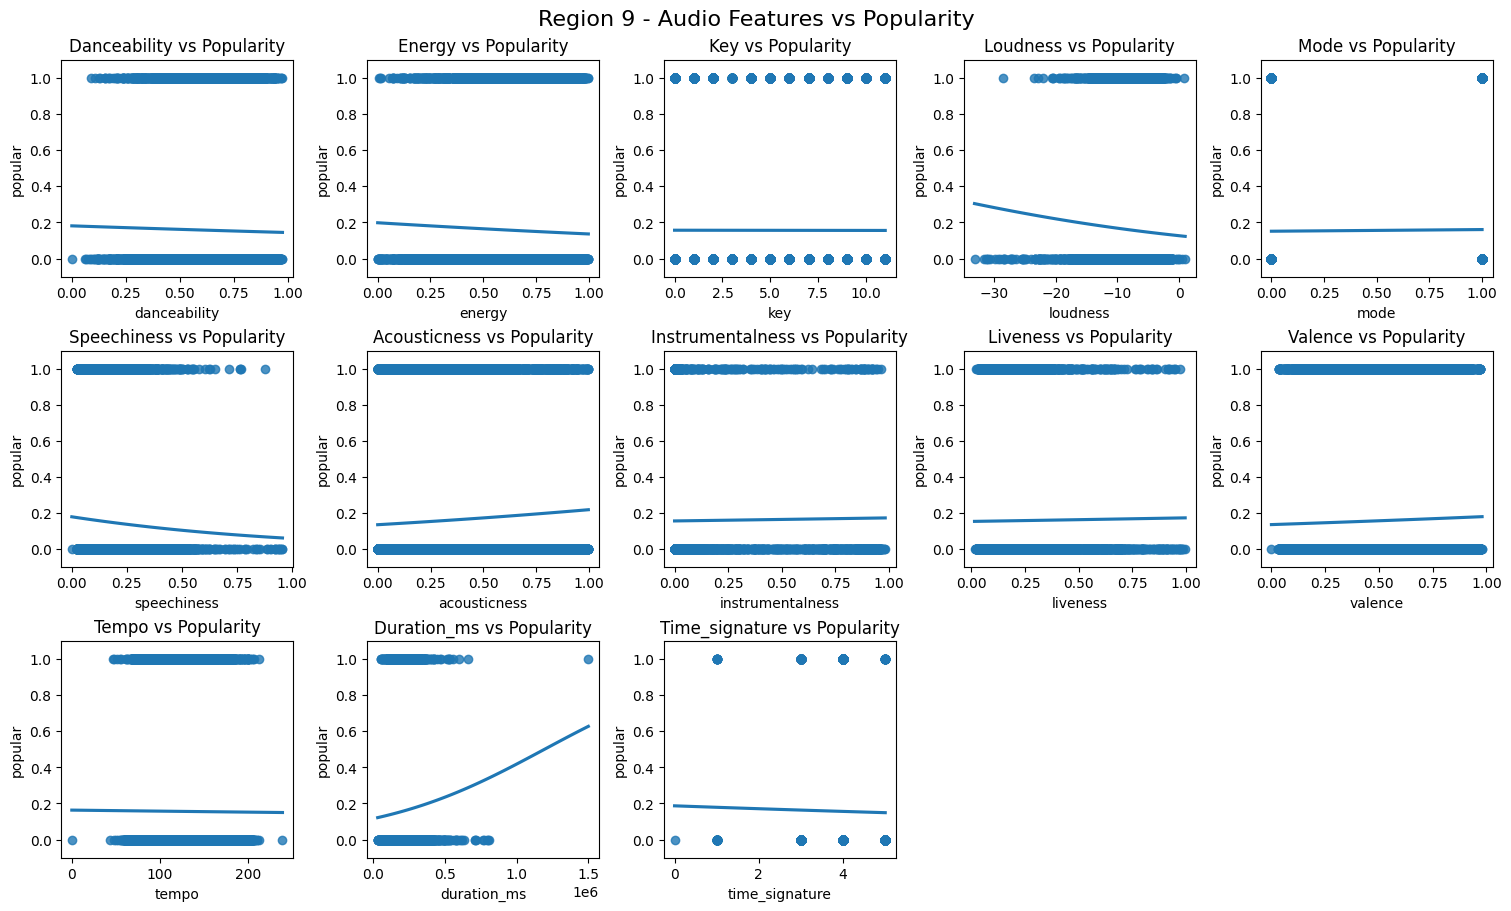
\includegraphics[width=\linewidth]{media/region9_cleaned.png}
        \caption{Popularity in Southern Europe}
        \label{southern_europe}
    \end{minipage}
    
    \vspace{0.05\textwidth}
    
    \begin{minipage}{0.45\textwidth}
        \centering
        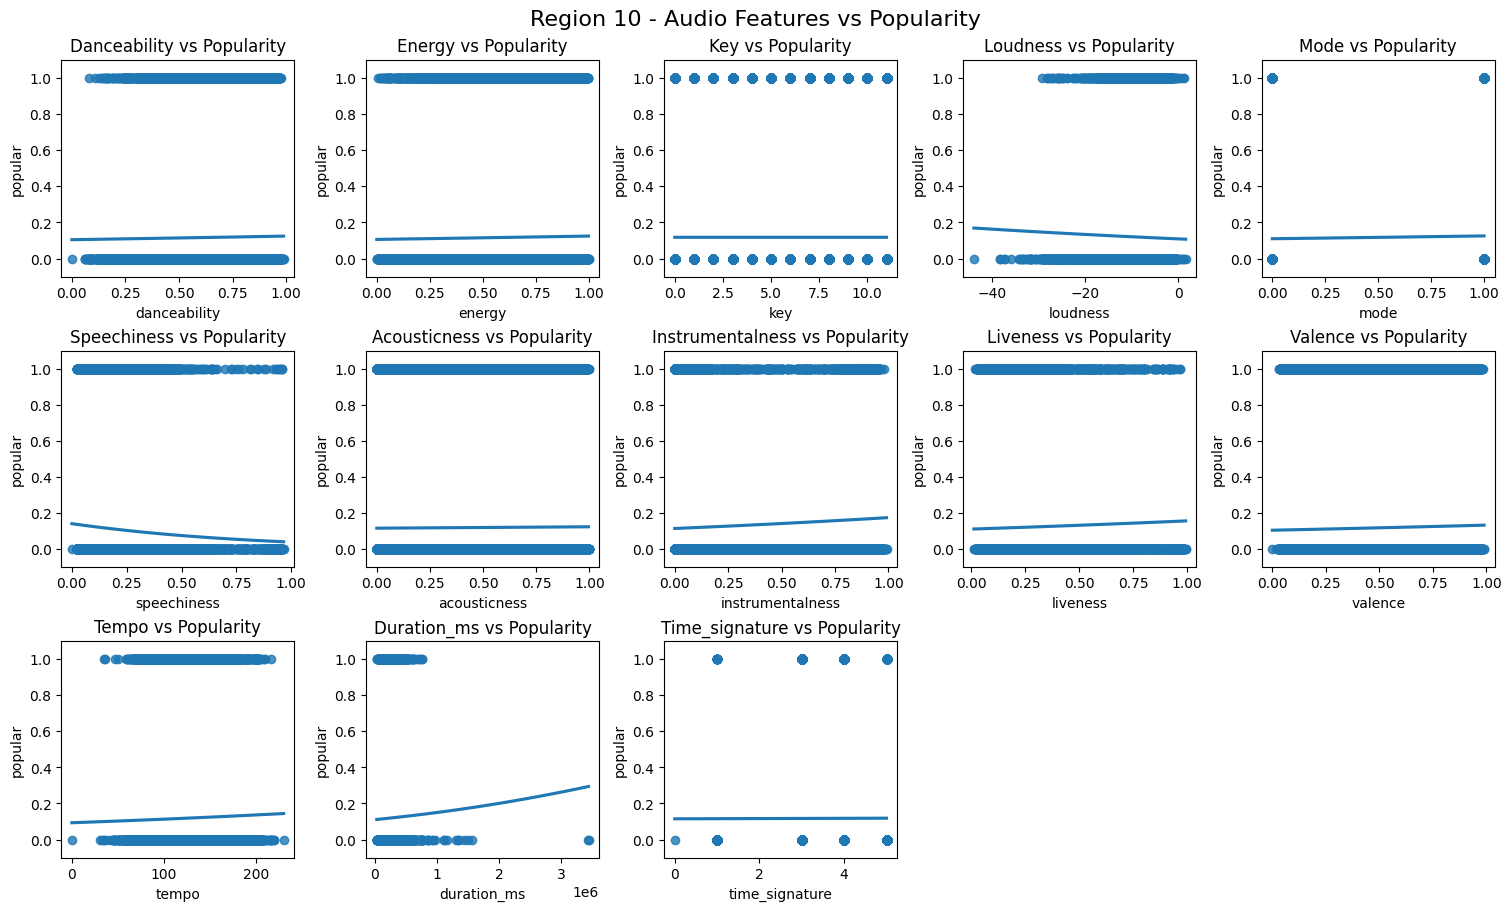
\includegraphics[width=\linewidth]{media/region10_cleaned.png}
        \caption{Popularity in Western Europe}
        \label{western_europe}
    \end{minipage}%
    \hspace{0.05\textwidth}
    \begin{minipage}{0.45\textwidth}
        \centering
        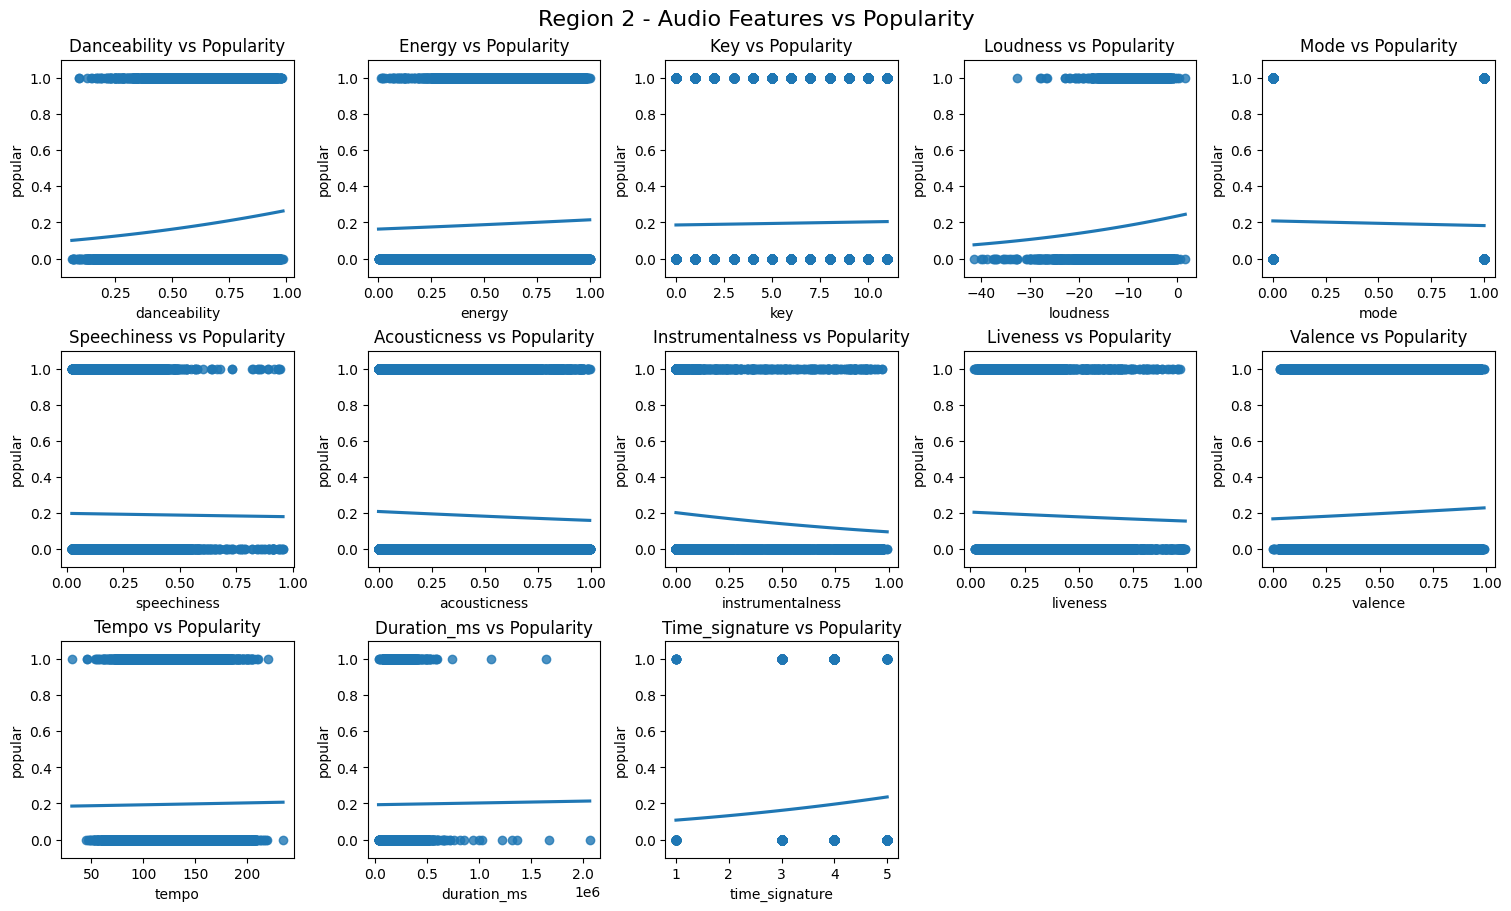
\includegraphics[width=\linewidth]{media/region2_cleaned.png}
        \caption{Popularity in Eastern Europe}
        \label{eastern_europe}
    \end{minipage}
    
    \vspace{0.05\textwidth}
    
    \begin{minipage}{0.45\textwidth}
        \centering
        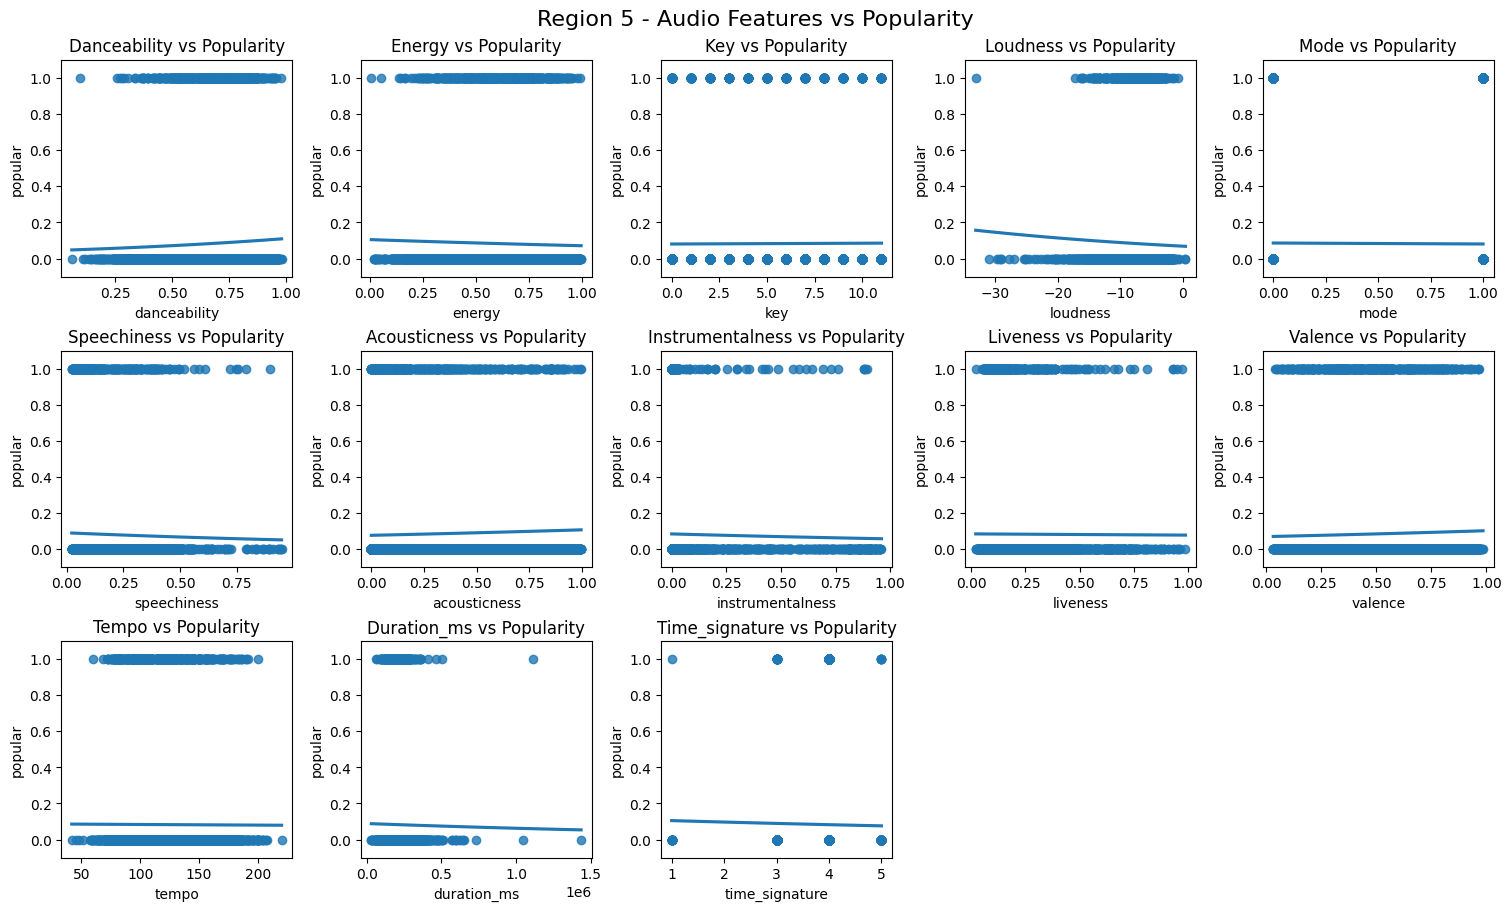
\includegraphics[width=\linewidth]{media/region5_cleaned.png}
        \caption{Popularity in North America}
        \label{north_america}
    \end{minipage}%
    \hspace{0.05\textwidth}
    \begin{minipage}{0.45\textwidth}
        \centering
        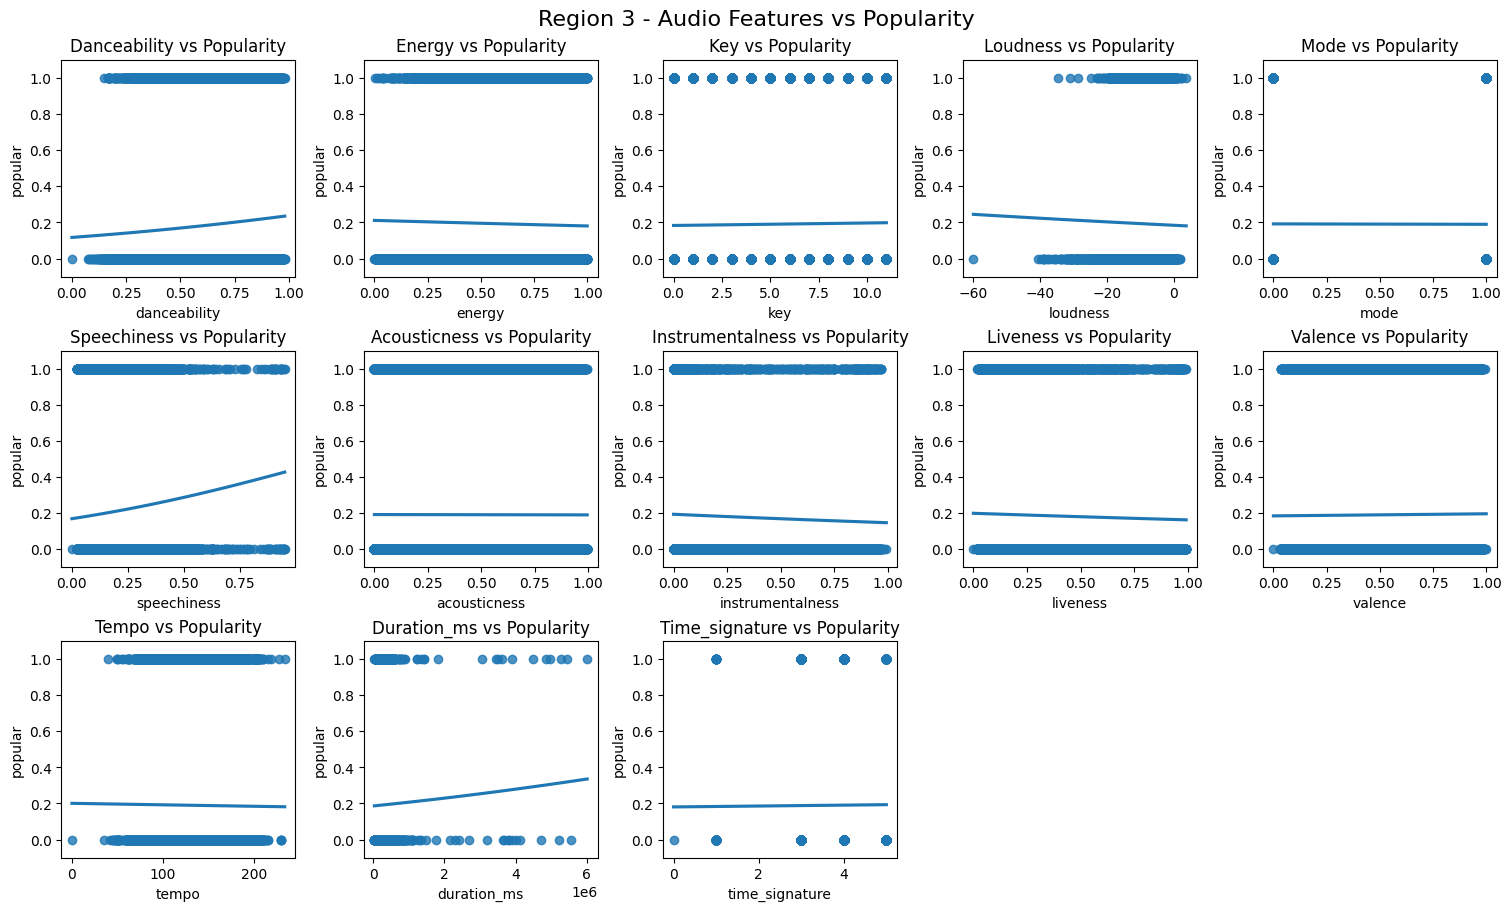
\includegraphics[width=\linewidth]{media/region3_cleaned.png}
        \caption{Popularity in Latin America}
        \label{latin_america}
    \end{minipage}
\end{figure}

\clearpage % Force new page after 6 figures

\begin{figure}[h]
    \centering
    \begin{minipage}{0.45\textwidth}
        \centering
        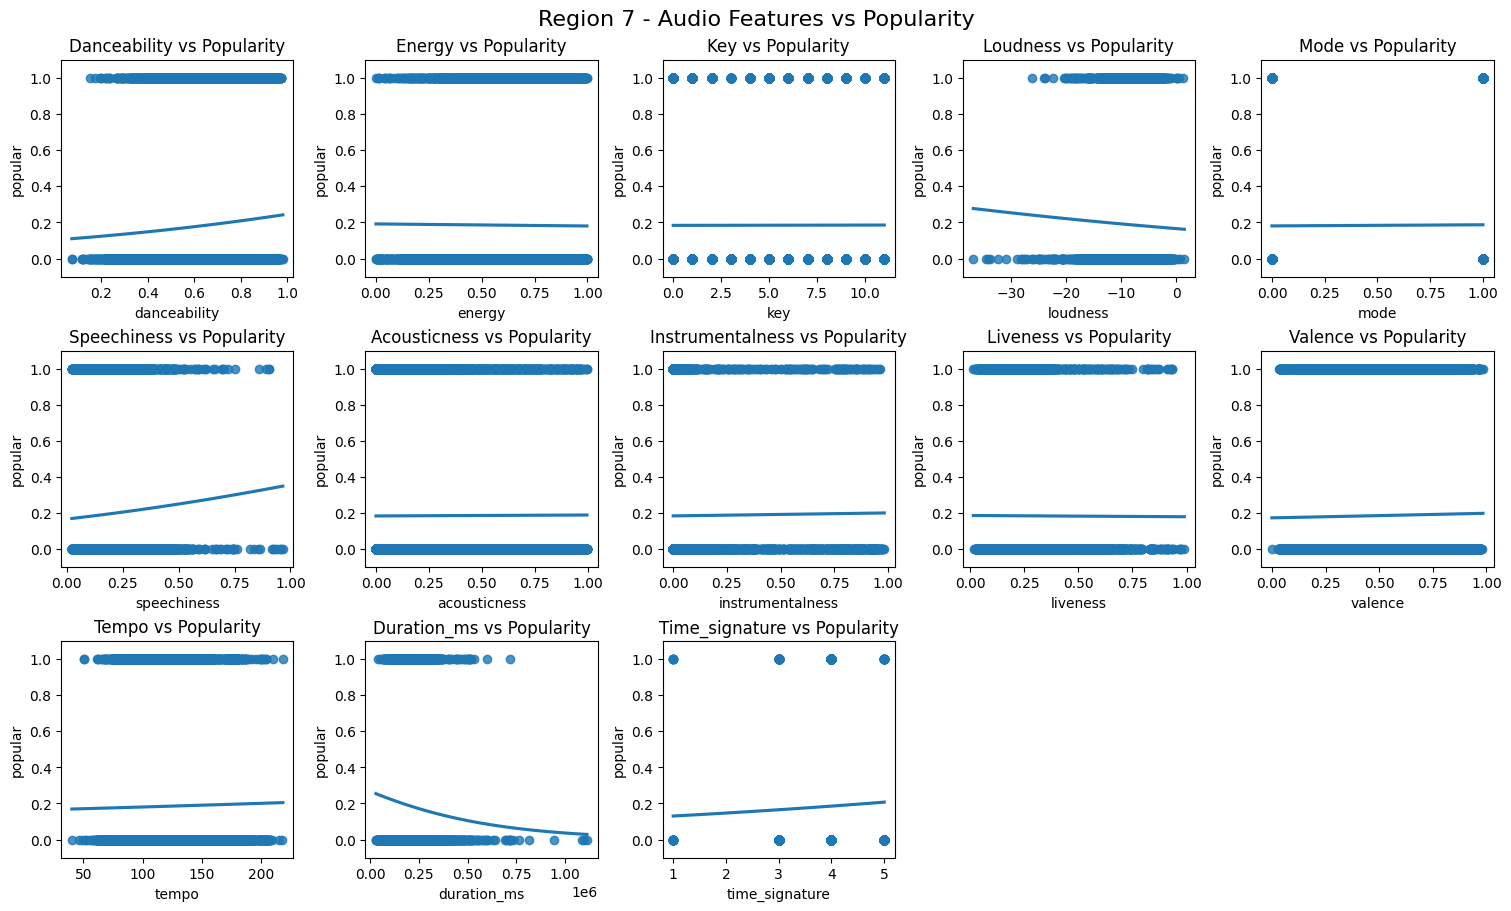
\includegraphics[width=\linewidth]{media/region7_cleaned.png}
        \caption{Popularity in Oceania}
        \label{oceania}
    \end{minipage}%
    \hspace{0.05\textwidth}
    \begin{minipage}{0.45\textwidth}
        \centering
        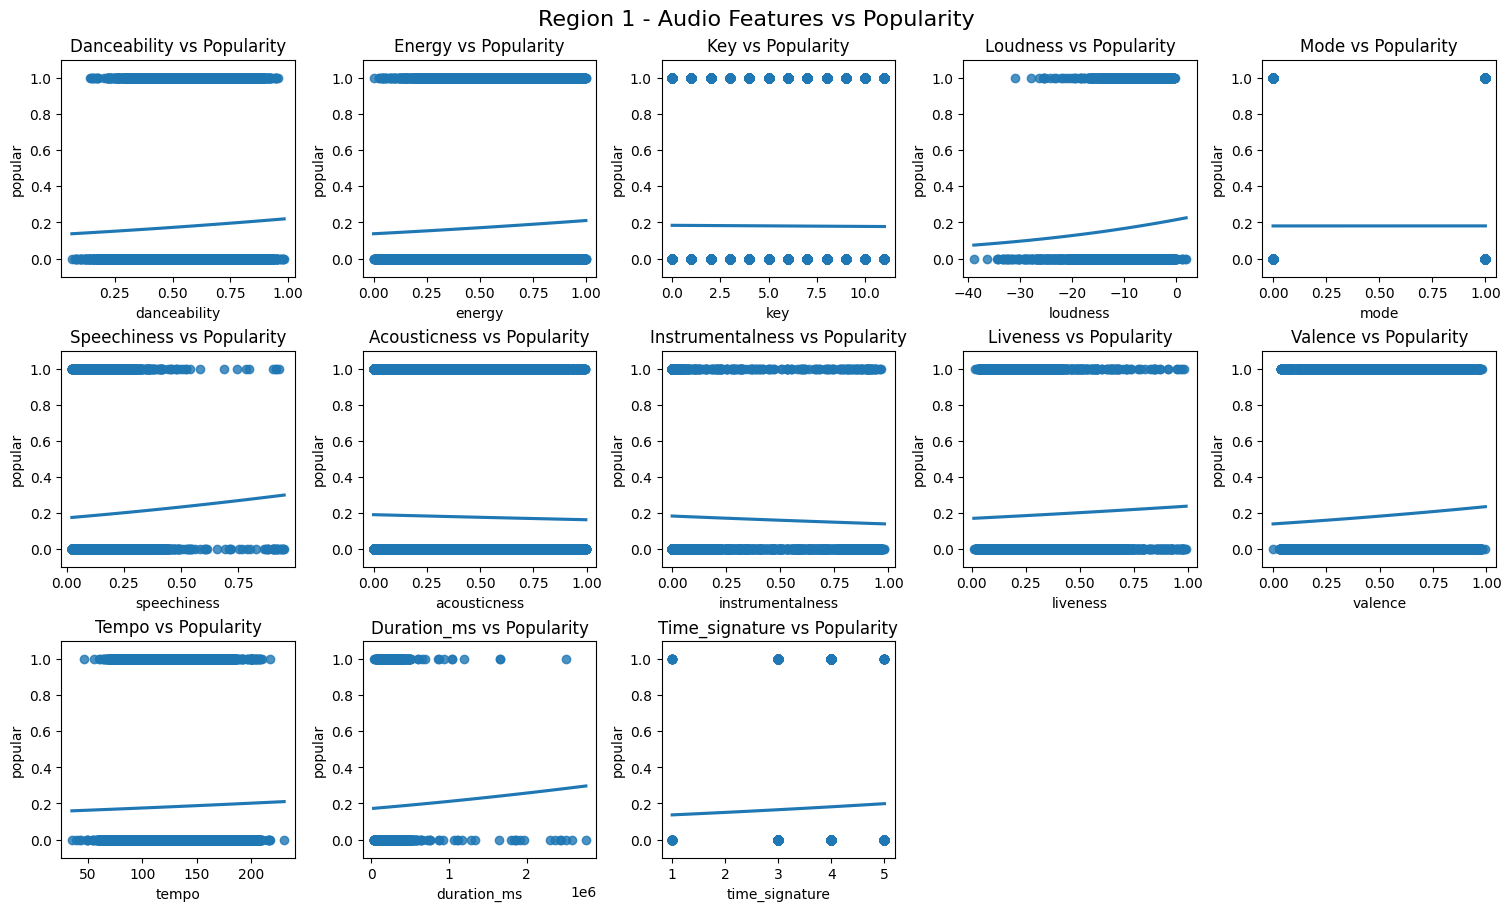
\includegraphics[width=\linewidth]{media/region1_cleaned.png}
        \caption{Popularity in East Asia}
        \label{east_asia}
    \end{minipage}
    
    \vspace{0.05\textwidth}
    
    \begin{minipage}{0.45\textwidth}
        \centering
        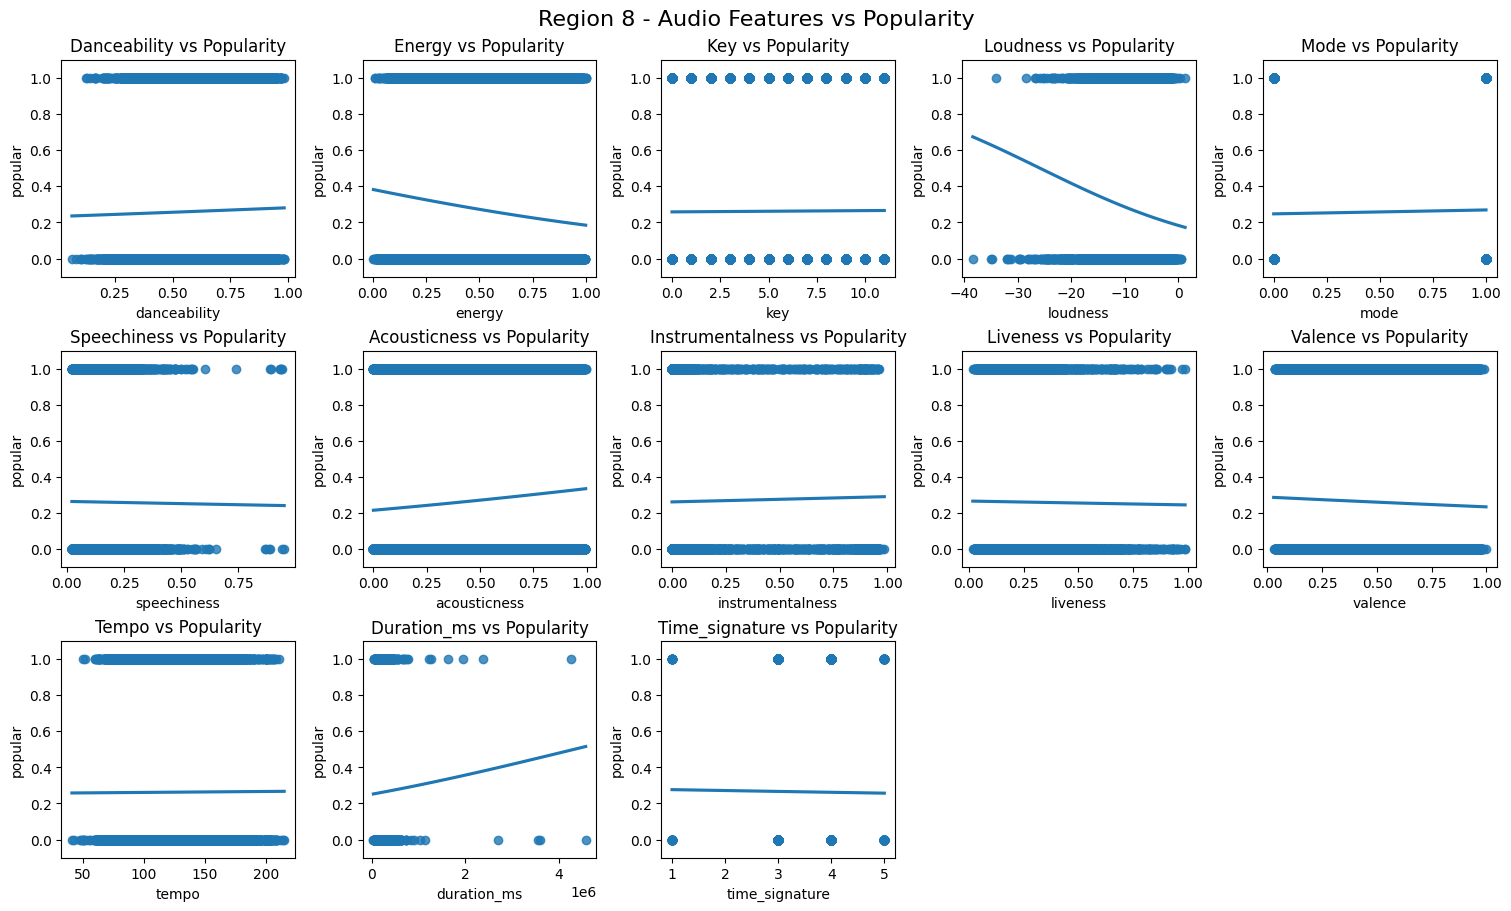
\includegraphics[width=\linewidth]{media/region8_cleaned.png}
        \caption{Popularity in South Asia}
        \label{south_asia}
    \end{minipage}%
    \hspace{0.05\textwidth}
    \begin{minipage}{0.45\textwidth}
        \centering
        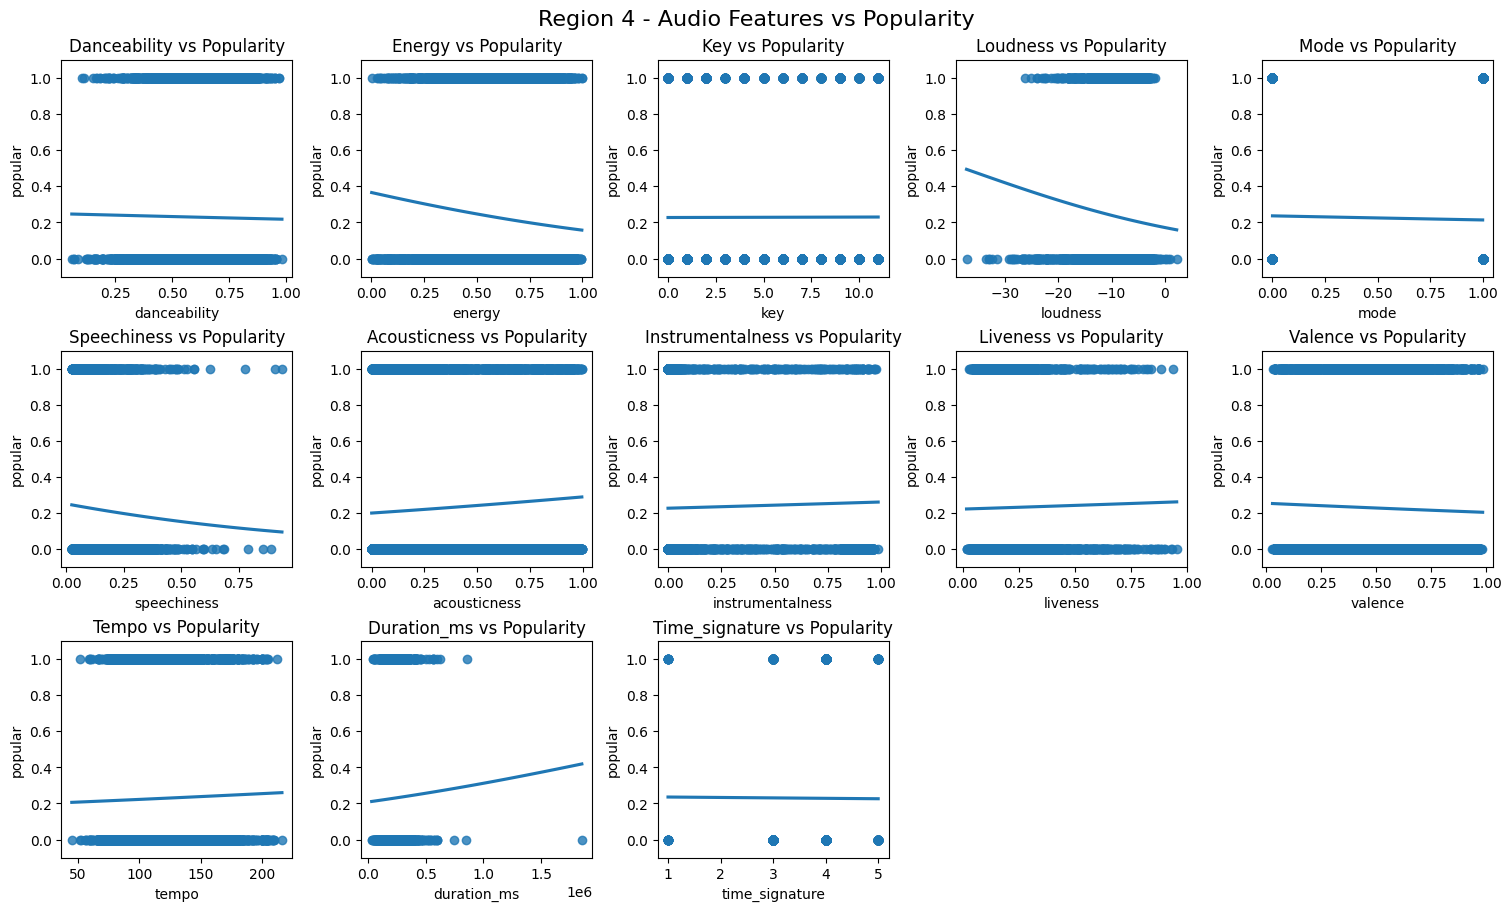
\includegraphics[width=\linewidth]{media/region4_cleaned.png}
        \caption{Popularity in the Middle East}
        \label{middle_east}
    \end{minipage}
\end{figure}

\begin{figure}[h]
    \centering
    \begin{minipage}{0.45\textwidth}
        \centering
        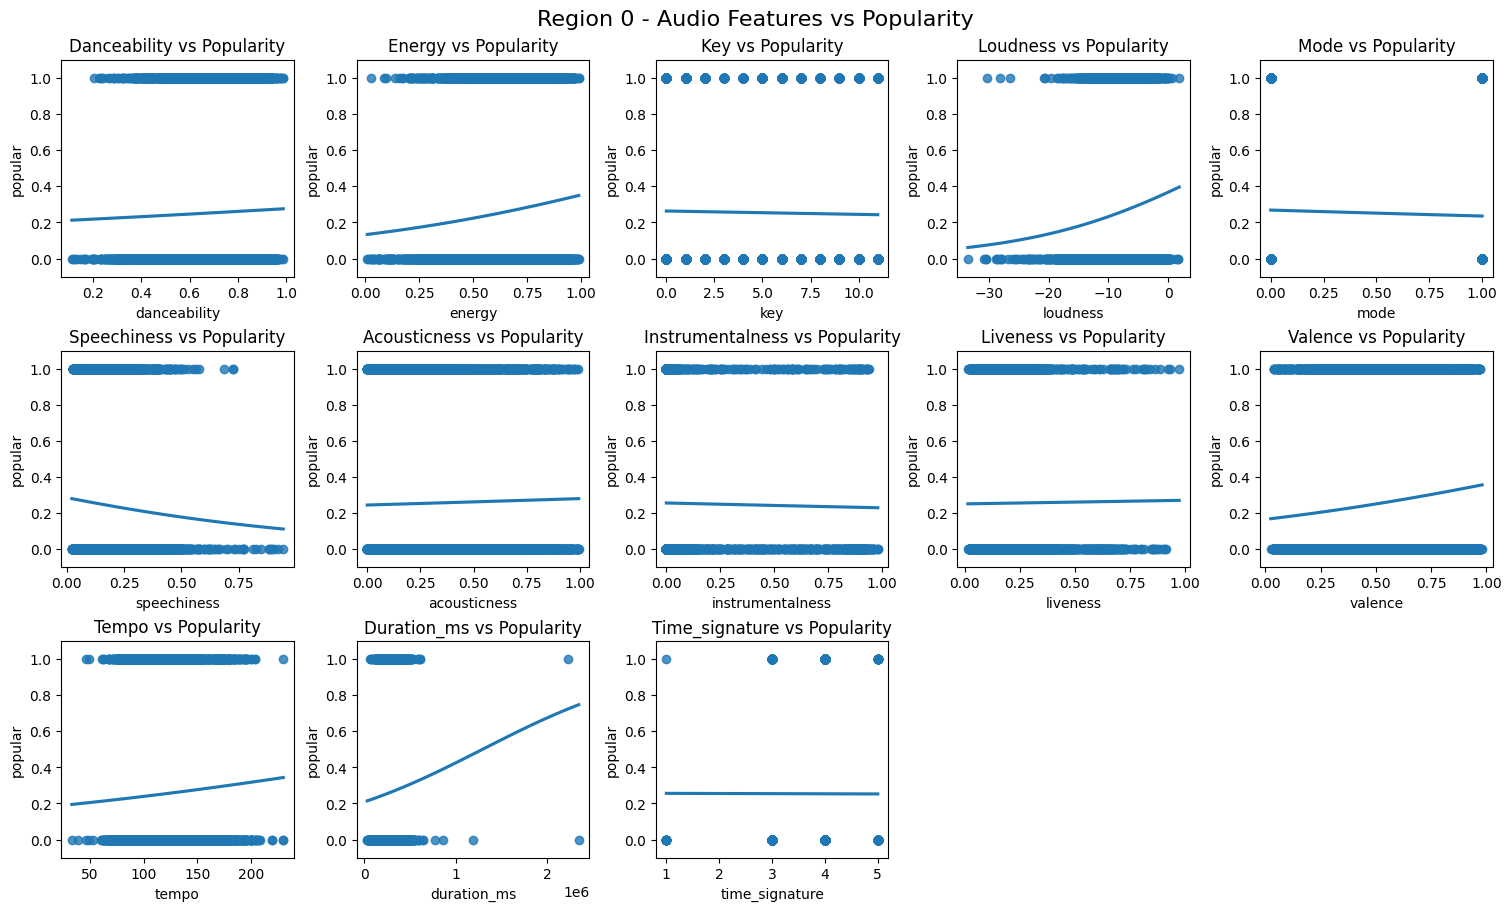
\includegraphics[width=\linewidth]{media/region0_cleaned.png}
        \caption{Popularity in Africa}
        \label{africa}
    \end{minipage}
\end{figure}


This allows us to understand what features make a song popular or not in the different regions.

\begin{itemize}
    \item \textbf{Northern Europe}: energy and danceability
    \item \textbf{Southern Europe}: acousticness and valence
    \item \textbf{Eastern Europe}: danceability
    \item \textbf{North America}: danceability and acousticness
    \item \textbf{Latin America}: speechiness and danceability
    \item \textbf{Oceania}: danceability and energy
    \item \textbf{East Asia}: valence
    \item \textbf{South Asia}: danceability and acousticness
    \item \textbf{Middle East}: danceability
    \item \textbf{Africa}: loudness, valence, acousticness, duration and tempo
    
\end{itemize}
   

\begin{figure}[H]
    \centering
    \begin{minipage}{0.45\textwidth}
        \centering
        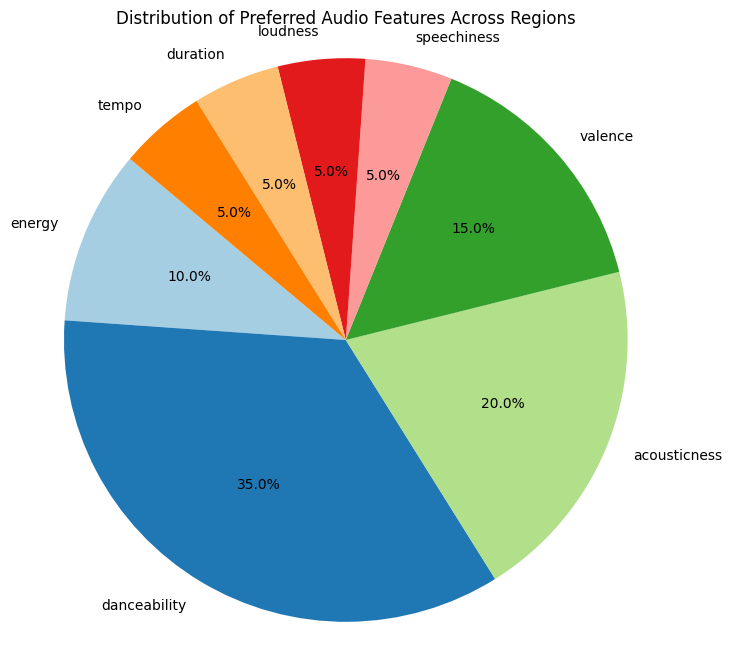
\includegraphics[width=\textwidth]{media/features_preferences.png}  
        \caption{Global preferences}
    \end{minipage}
    \hfill
    \begin{minipage}{0.54\textwidth}
        \centering
        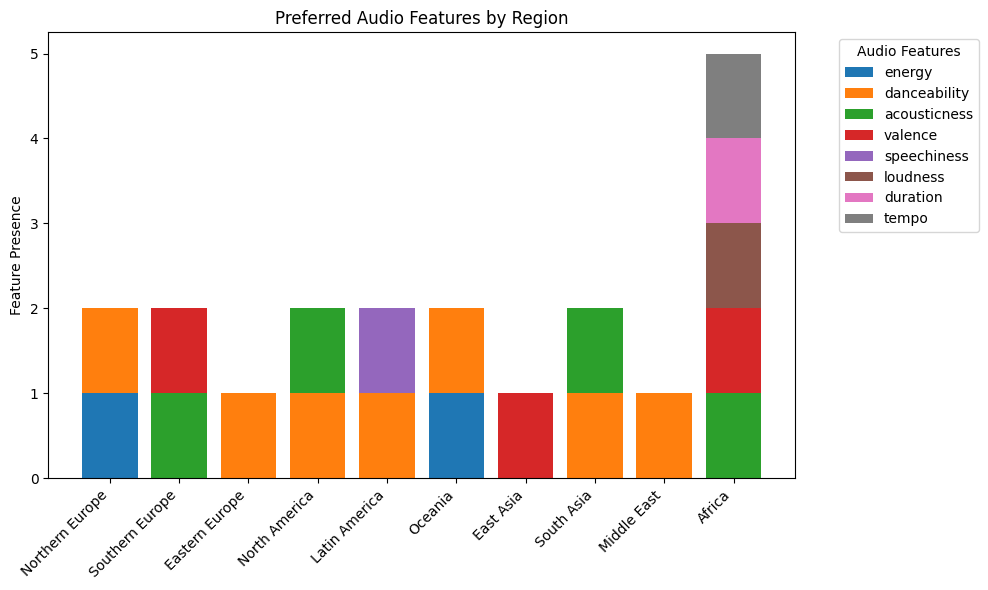
\includegraphics[width=\textwidth]{media/feature_preferences_regions.png}  
        \caption{Regional preferences}
    \end{minipage}
\end{figure}


\chapter{Algorithms}
%maybe a small introduction to algorithms about why we chose these algorithms

\section{Logistic Regression}
Logistic regression is one of the supervised machine learning algorithms to
compute classification problems. It is used to predict the probability of a
categorical dependent variable. In this project's case, logistic regression is used to predict
whether a song will be popular or not depends on where it will be released and the 
audio features of the song. Logistic regression is a statistical method for 
predicting binary outcomes from the data. The output of the logistic regression is values
either 0 or 1, which 0 represents the song most probably will not be popular and 
1 represents the song most probably will be popular. \\

\subsection{Implementation Steps}
\begin{itemize}
    \item \textbf{Data Preparation: } The dataset was split into X as all the audio features and region and Y as popular.
    The popular column used as the target variable. Then the dataset is split into training and testing sets using an 80-20 split.
    \item \textbf{Feature Scaling: } Features were scaled using the \textit{StandardScaler} from the \textit{sklearn.preprocessing} library to 
    normalize the data and to ensure that all feautres contribute equally to the distance calculation involved in the model, which helps improve the convergence of the algorithm.
    \item \textbf{Handling Class Imbalancae: } To address potential class imbalance in the dataset, the \textit{Synthetic Minority Over-sampling Technique (SMOTE)} was applied, which
    created synthetic samples of the minorty class (popular songs).
    \item \textbf{Model Training: } The logistic regression model was trained using the scaled training set. The model was
    configured with a maximum iteration limit of 2000 and class weight balanced to give equal importance to both classes during the training.
    \item \textbf{Cross-Validation: } To evaluate the model's performance more robustly, 5-fold cross-validation was performed.
    This technique involves splitting the data into five subsets (folds) and training the model on four folds while validating it on the remaining
    fold. This process is repeated five times, each time using a different fold for validation.
        \begin{figure}[h] 
            \centering 
            
\includegraphics[width=0.6\textwidth]{media/logistic_reg_cross_val_results.png} 
        \end{figure}
    \item \textbf{Predictions: } Predictions were made on the scaled test set, and probabilities were calculated for class membership. A threshold of 0.3 was used to adjust the predicted probabilities to determine class labels.
    \item \textbf{Model Evaluation: } The model was evaluated using the confusion matrix, classification report, which included metrics such as precicion, recall, and F1-score.
        \begin{figure}[h] 
            \centering 
            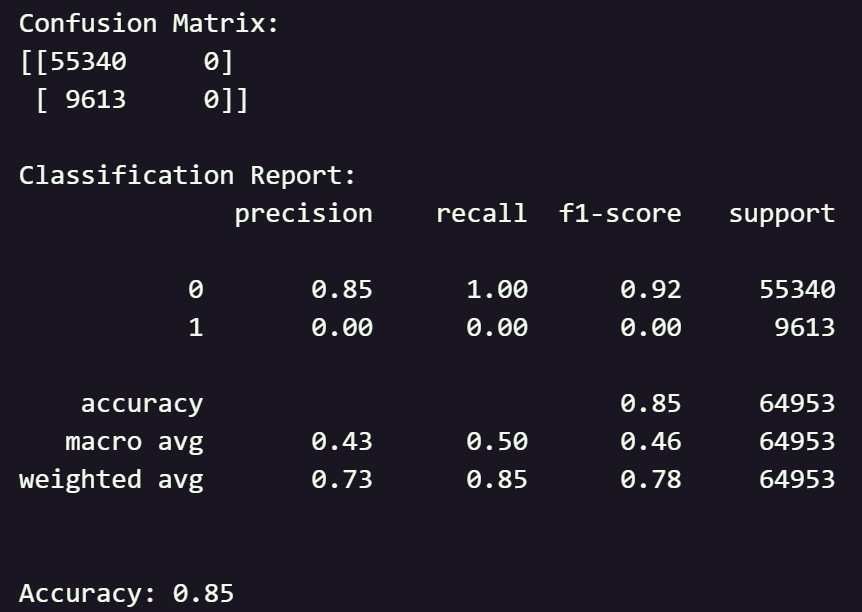
\includegraphics[width=0.35\textwidth]{media/logistic_reg_results.png} 
        \end{figure}
        \\
        \textbf{Confusion Matrix: }
        \begin{itemize}
            \item True Negatives (TN): 55,340 - The model correctly predicted that 55,340 songs are not popular (class 0).
            \item False Negatives (FN): 9,613 - The model incorrectly predicted that 9,613 popular songs (class 1) are not popular.
            \item True Positives (TP): 0 - The model did not correctly identify any songs as popular.
            \item False Positives (FP): 0 - The model did not incorrectly predict any songs as popular.
        \end{itemize}
        
        \textbf{Classification Report: }
        \begin{itemize}
            \item Precision: 
                \begin{itemize}
                    \item Class 0 (not popular): 0.85 - Among the predicted non-popular songs, 85\% were correctly identified.
                    \item Class 1 (popular): 0.0 - The model did not correctly identify any popular songs, resulting in a precision of 0.
                \end{itemize}
            \item Recall:
                \begin{itemize}
                    \item Class 0 (not popular): 1.00 - The model perfectly identified all non-popular songs (no false negatives).
                    \item Class 1 (popular): 0.0 - The model failed to identify any popular songs (no true positives).

                \end{itemize}
            \item F1-Score:
                \begin{itemize}
                    \item Class 0 (not popular): 0.92 - A high F1-score indicates a good balance between precision and recall for non-popular songs.
                    \item Class 1 (popular): 0.0 - Since there are no true positives, the F1-score is also 0.
                \end{itemize}
        \end{itemize}
        \textbf{Overall Acuracy: } 
        \\
        0.85 - The overall accuracy of the model is 85\%. However, this number is misleading in the context of a highly imbalanced dataset, as it reflects the model's ability to predict the majority class (not popular) rather than its performance on both classes.
    \item \textbf{Feature Importance: } The feature importance of the model was determined by examining the coefficients of the logistic regression model. Both feature importance for whole dataset and feature importance for each specific region has been applied. As a result of this dominant features to determine populartiy of the songs were found.
        \begin{figure}[h] 
            \centering 
            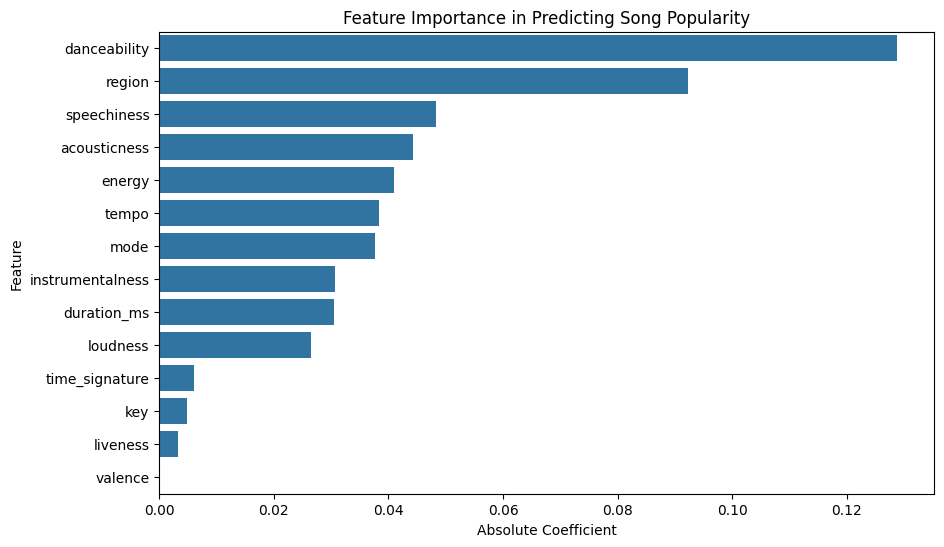
\includegraphics[width=0.7\textwidth]{media/logistic_reg_feature_imp.png} 
        \end{figure}
        \textbf{Feature Importance for Regions Examples: }
        \begin{figure}[h] 
            \centering 
            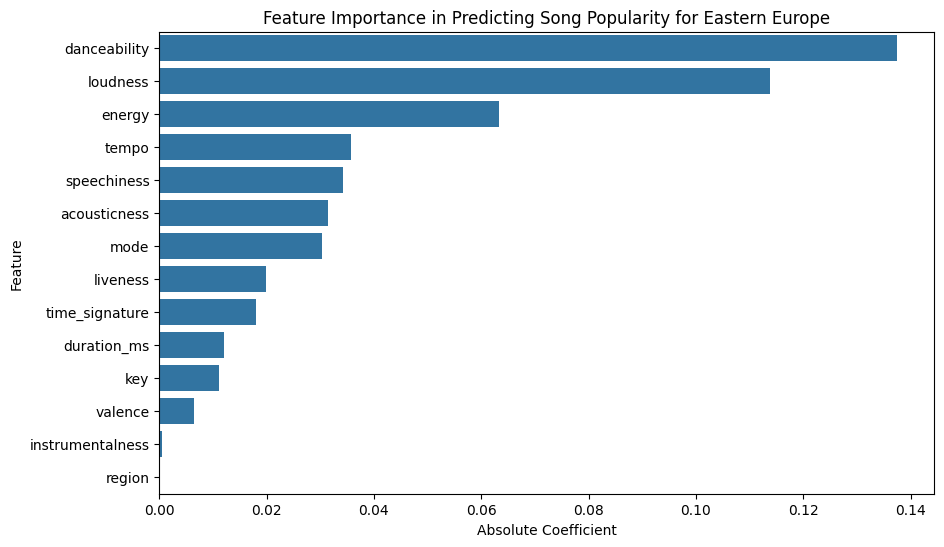
\includegraphics[width=0.7\textwidth]{media/log_reg_feature_selection_eastern_europe.png} 
        \end{figure}
        \begin{figure}[h] 
            \centering 
            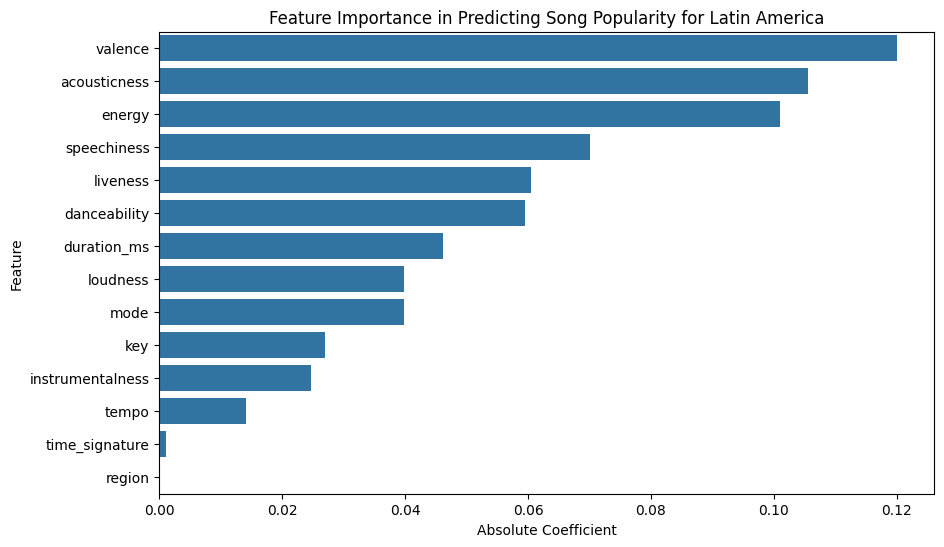
\includegraphics[width=0.7\textwidth]{media/log_reg_feature_selection_latin_america.png} 
        \end{figure}
    \item \textbf{Regional Analysis: } Regional analysis was performed to better understand how different audio features contribute to song populartiy across various regions.
    \begin{table}[ht]
        \centering
        \begin{adjustbox}{width=\textwidth}
        \begin{tabular}{lrrrrrrrrrrrrrrrr}
        \toprule
        Region & Rank\_Mean & Frequency & Danceability & Energy & Key & Loudness & Mode & Speechiness & Acousticness & Instrumentalness & Liveness & Valence & Tempo & Duration\_ms & Time\_Signature & Popular \\
        \midrule
        0  & 77.28 & 51.34 & 0.686 & 0.620 & 5.21 & -7.61 & 0.507 & 0.138 & 0.259 & 0.042 & 0.168 & 0.484 & 120.41 & 219551.52 & 3.96 & 0.157 \\
        1  & 76.33 & 49.11 & 0.603 & 0.629 & 5.29 & -6.86 & 0.678 & 0.080 & 0.303 & 0.042 & 0.177 & 0.471 & 121.52 & 229571.73 & 3.96 & 0.117 \\
        2  & 69.78 & 79.65 & 0.661 & 0.641 & 5.29 & -7.34 & 0.541 & 0.130 & 0.241 & 0.056 & 0.182 & 0.471 & 122.33 & 205515.98 & 3.96 & 0.181 \\
        3  & 71.24 & 188.65 & 0.663 & 0.660 & 5.36 & -6.71 & 0.593 & 0.106 & 0.286 & 0.042 & 0.194 & 0.581 & 122.61 & 217127.50 & 3.94 & 0.184 \\
        4  & 75.45 & 61.90 & 0.642 & 0.611 & 5.29 & -7.63 & 0.462 & 0.105 & 0.295 & 0.057 & 0.178 & 0.470 & 120.14 & 213894.57 & 3.95 & 0.152 \\
        5  & 79.72 & 49.95 & 0.658 & 0.620 & 5.19 & -6.99 & 0.610 & 0.131 & 0.237 & 0.031 & 0.179 & 0.464 & 121.36 & 206987.98 & 3.95 & 0.127 \\
        6  & 78.48 & 50.92 & 0.642 & 0.636 & 5.32 & -7.35 & 0.563 & 0.109 & 0.232 & 0.044 & 0.182 & 0.486 & 121.29 & 203514.75 & 3.95 & 0.120 \\
        7  & 67.06 & 61.44 & 0.647 & 0.631 & 5.22 & -7.05 & 0.608 & 0.116 & 0.231 & 0.048 & 0.179 & 0.472 & 120.82 & 213396.98 & 3.96 & 0.163 \\
        8  & 71.30 & 98.99 & 0.623 & 0.584 & 5.24 & -7.39 & 0.659 & 0.082 & 0.359 & 0.035 & 0.172 & 0.460 & 119.92 & 222230.31 & 3.94 & 0.197 \\
        9  & 71.92 & 52.77 & 0.649 & 0.646 & 5.31 & -7.02 & 0.564 & 0.119 & 0.265 & 0.041 & 0.177 & 0.496 & 121.24 & 210862.34 & 3.95 & 0.125 \\
        10 & 81.34 & 64.66 & 0.669 & 0.643 & 5.34 & -7.26 & 0.525 & 0.145 & 0.252 & 0.056 & 0.173 & 0.489 & 120.90 & 205864.40 & 3.96 & 0.117 \\
        \bottomrule
        \end{tabular}
        \end{adjustbox}
        \end{table}
\end{itemize} 







\section{Decision Tree}




\section{Random Forest}
Random Forest is an ensemble learning method that constructs a multitude of decision trees during
training and outputs the mode of the classes as the prediction of the individual trees. Random Forest
is a versatile machine learning algorithm that can be used for both classification and regression
tasks. It is based on the concept of bagging, which involves training multiple models on different
subsets of the data and combining their predictions to improve the overall performance. Random Forest
is known for its robustness, scalability, and ability to handle high-dimensional data with ease.
In this project, Random Forest was used to predict whether the song will be popular or not based on their audio
features and release region. \\

\subsection{Implementation Steps}
\begin{itemize}
    \item \textbf{Data Preparation: } 
    \item \textbf{Feature Scaling: } 
    \item \textbf{Handling Class Imbalancae: } 
    \item \textbf{Model Training: } 
    \item \textbf{Cross-Validation: } 
        \begin{figure}[h] 
            \centering 
            
\includegraphics[width=0.6\textwidth]{media/random_forest_cross_validation.png} 
        \end{figure}
    \item \textbf{Predictions: } 
    \item \textbf{Model Evaluation: } 
        \begin{figure}[h] 
            \centering 
            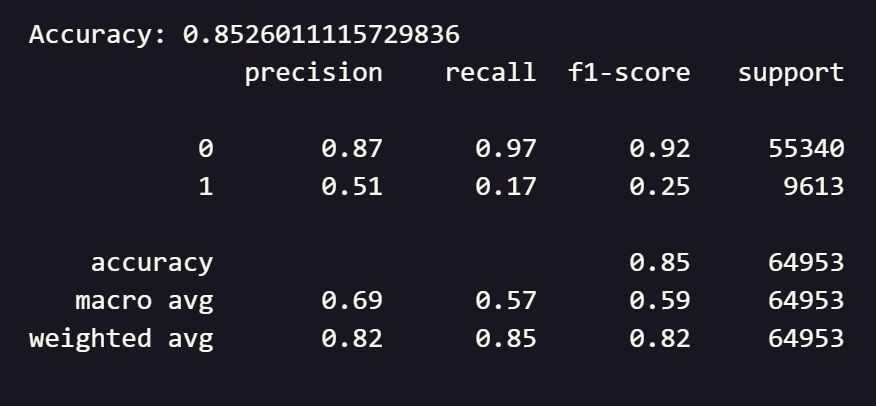
\includegraphics[width=0.35\textwidth]{media/random_forest_accuracy_numbers.png} 
        \end{figure}
        \\
        \textbf{Confusion Matrix: }
        \begin{figure}[h] 
            \centering 
            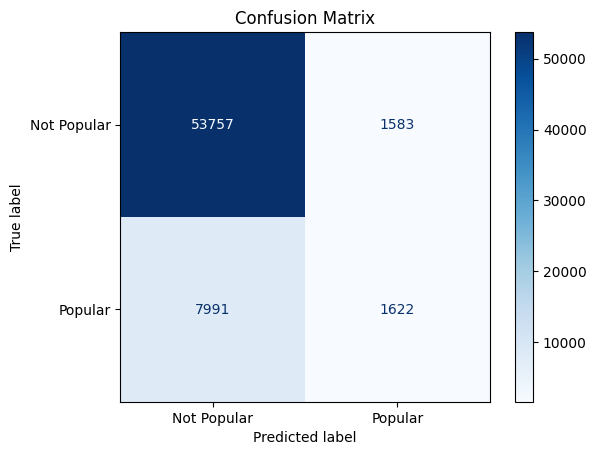
\includegraphics[width=0.35\textwidth]{media/random_forest_conf_matrix.png} 
        \end{figure}
        \begin{itemize}
            \item True Negatives (TN): 55,340 
            \item False Negatives (FN): 9,613 
            \item True Positives (TP): 0 
            \item False Positives (FP): 0 
        \end{itemize}
        
        \textbf{Classification Report: }
        \begin{itemize}
            \item Precision: 
                \begin{itemize}
                    \item Class 0 (not popular): 0.85 - Among the predicted non-popular songs, 85\% were correctly identified.
                    \item Class 1 (popular): 0.0 - The model did not correctly identify any popular songs, resulting in a precision of 0.
                \end{itemize}
            \item Recall:
                \begin{itemize}
                    \item Class 0 (not popular): 1.00 - The model perfectly identified all non-popular songs (no false negatives).
                    \item Class 1 (popular): 0.0 - The model failed to identify any popular songs (no true positives).

                \end{itemize}
            \item F1-Score:
                \begin{itemize}
                    \item Class 0 (not popular): 0.92 - A high F1-score indicates a good balance between precision and recall for non-popular songs.
                    \item Class 1 (popular): 0.0 - Since there are no true positives, the F1-score is also 0.
                \end{itemize}
        \end{itemize}
        \textbf{Overall Acuracy: } 
        \\
        0.85 - The overall accuracy of the model is 85\%. However, this number is misleading in the context of a highly imbalanced dataset, as it reflects the model's ability to predict the majority class (not popular) rather than its performance on both classes.
    \item \textbf{Feature Importance: } 
        \begin{figure}[h] 
            \centering 
            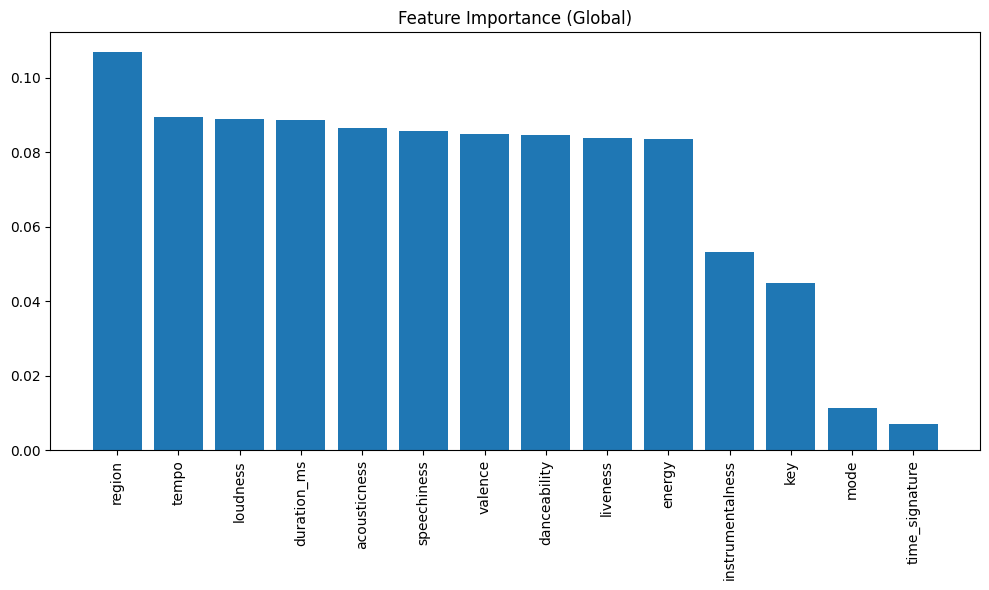
\includegraphics[width=0.7\textwidth]{media/random_forest_feature_importance.png} 
        \end{figure}
        \textbf{Feature Importance for Regions Examples: }
        \begin{figure}[h] 
            \centering 
            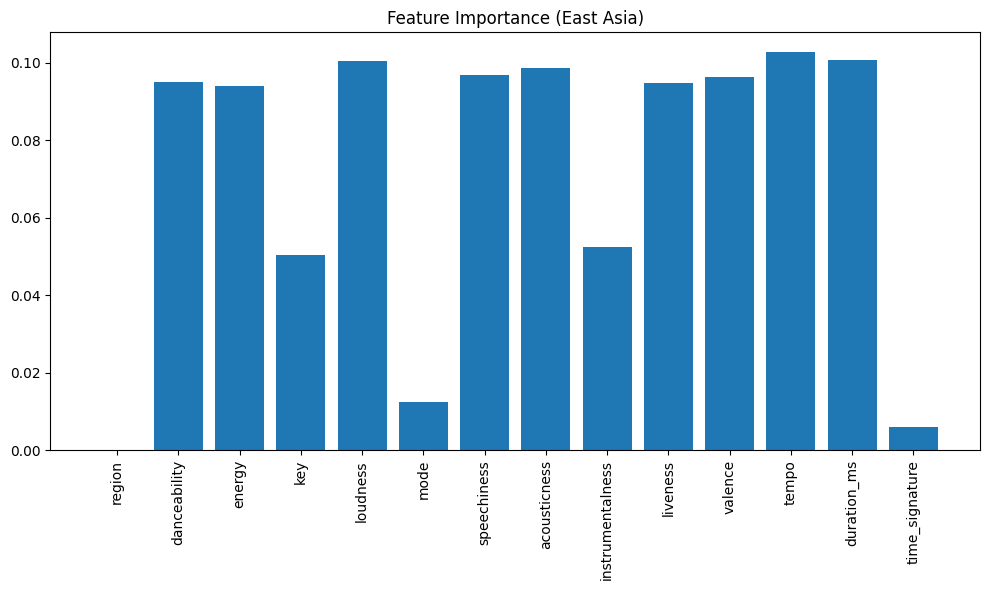
\includegraphics[width=0.7\textwidth]{media/random_forest_feature_imp_east_asia.png} 
        \end{figure}
        \begin{figure}[h] 
            \centering 
            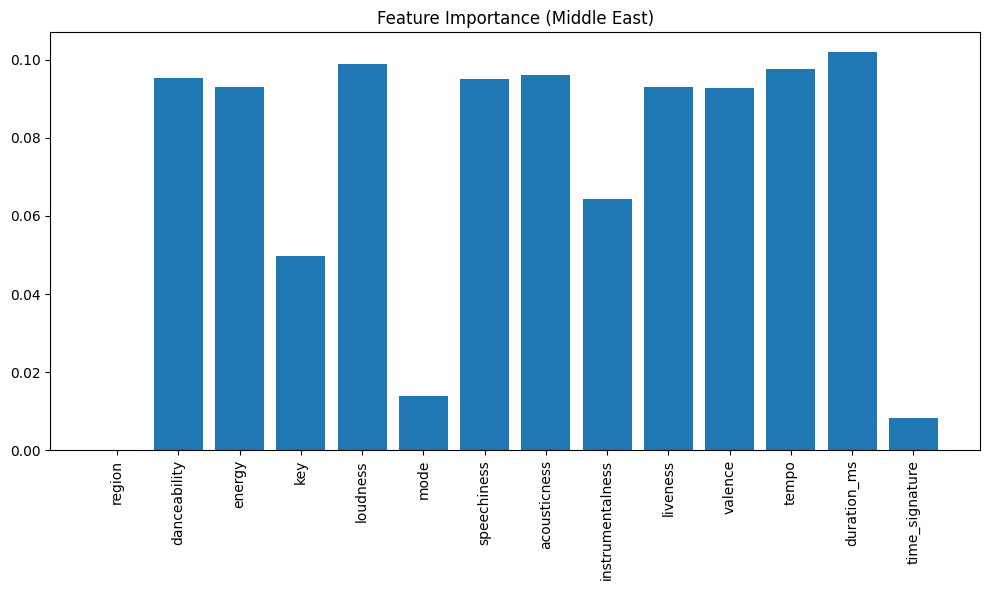
\includegraphics[width=0.7\textwidth]{media/random_forest_feature_imp_middle_east.png} 
        \end{figure}
    \item \textbf{Regional Analysis: } 
    \begin{table}[ht]
        \centering
        \begin{adjustbox}{width=\textwidth}
        \begin{tabular}{lrrrrrrrrrrrrrrrr}
        \toprule
        Region & Rank\_Mean & Frequency & Danceability & Energy & Key & Loudness & Mode & Speechiness & Acousticness & Instrumentalness & Liveness & Valence & Tempo & Duration\_ms & Time\_Signature & Popular \\
        \midrule
        0  & 77.28 & 51.34 & 0.686 & 0.620 & 5.21 & -7.61 & 0.507 & 0.138 & 0.259 & 0.042 & 0.168 & 0.484 & 120.41 & 219551.52 & 3.96 & 0.157 \\
        1  & 76.33 & 49.11 & 0.603 & 0.629 & 5.29 & -6.86 & 0.678 & 0.080 & 0.303 & 0.042 & 0.177 & 0.471 & 121.52 & 229571.73 & 3.96 & 0.117 \\
        2  & 69.78 & 79.65 & 0.661 & 0.641 & 5.29 & -7.34 & 0.541 & 0.130 & 0.241 & 0.056 & 0.182 & 0.471 & 122.33 & 205515.98 & 3.96 & 0.181 \\
        3  & 71.24 & 188.65 & 0.663 & 0.660 & 5.36 & -6.71 & 0.593 & 0.106 & 0.286 & 0.042 & 0.194 & 0.581 & 122.61 & 217127.50 & 3.94 & 0.184 \\
        4  & 75.45 & 61.90 & 0.642 & 0.611 & 5.29 & -7.63 & 0.462 & 0.105 & 0.295 & 0.057 & 0.178 & 0.470 & 120.14 & 213894.57 & 3.95 & 0.152 \\
        5  & 79.72 & 49.95 & 0.658 & 0.620 & 5.19 & -6.99 & 0.610 & 0.131 & 0.237 & 0.031 & 0.179 & 0.464 & 121.36 & 206987.98 & 3.95 & 0.127 \\
        6  & 78.48 & 50.92 & 0.642 & 0.636 & 5.32 & -7.35 & 0.563 & 0.109 & 0.232 & 0.044 & 0.182 & 0.486 & 121.29 & 203514.75 & 3.95 & 0.120 \\
        7  & 67.06 & 61.44 & 0.647 & 0.631 & 5.22 & -7.05 & 0.608 & 0.116 & 0.231 & 0.048 & 0.179 & 0.472 & 120.82 & 213396.98 & 3.96 & 0.163 \\
        8  & 71.30 & 98.99 & 0.623 & 0.584 & 5.24 & -7.39 & 0.659 & 0.082 & 0.359 & 0.035 & 0.172 & 0.460 & 119.92 & 222230.31 & 3.94 & 0.197 \\
        9  & 71.92 & 52.77 & 0.649 & 0.646 & 5.31 & -7.02 & 0.564 & 0.119 & 0.265 & 0.041 & 0.177 & 0.496 & 121.24 & 210862.34 & 3.95 & 0.125 \\
        10 & 81.34 & 64.66 & 0.669 & 0.643 & 5.34 & -7.26 & 0.525 & 0.145 & 0.252 & 0.056 & 0.173 & 0.489 & 120.90 & 205864.40 & 3.96 & 0.117 \\
        \bottomrule
        \end{tabular}
        \end{adjustbox}
        \end{table}
\end{itemize} 



\section{Naive Bayes}

\section{SVM}
\chapter{Literature Review}
%compare accuracy of the algorithms
%put global feature importance for each algorithm and compare them
%for the best algorithm, put feature importance for each region and compare them


\chapter{Results}

\section{Results of the Models}

\begin{table}[htbp]
    \centering
    \begin{tabular}{|l|c|c|}
    \hline
    \textbf{Model}           & \textbf{Accuracy} & \textbf{Weighted Average of Precision} \\ \hline
    Logistic Regression & 85.42\%          & 0.73                \\ \hline
    Decision Tree       & 75.97\%          & 0.77              \\ \hline
    Random Forests      & 85.67\%          & 0.83             \\ \hline
    Naïve Bayes         & 85.04\%          & 0.75               \\ \hline
    KNN                 & 83.92\%          & 0.80               \\ \hline
    \end{tabular}
    \caption{Accuracy and Weighted Average of Precision of Different Models}
    \end{table}
    
According to the results shown in the table above, Random Forests and Logistic Regression have the highest accuracy values. However Random Forests has 
higher value on weights Average of Precision
%what do you mean by "higher value on weights Average of Precision"?
and if the confusion matrixes are compared it can be shown that Random Forests has a higher 
probability of making correct predictions. This makes Random Forests the best model for this dataset with 85.67\% accuracy. 
In general, all the models have high accuracy values, which indicates that the dataset is well-suited for classification. Even the worst model, Decision Tree, has an accuracy of 75.97\%, which is still a high value.\\
Furthermore, our accuracy results are better than the article found in the literature, in which the best algorithm, Logistic Regression, had an accuracy of 52\%. This could be due to the fact that the dataset used in the literature was smaller and less diverse than the dataset used in this study.
\\

\section{Global Feature Importance Analysis}

It's important to understand the global importance of the features in the dataset to be able to make better predictions.

The Random Forest model shows that globally many features are important for predicting the popularity of a song: \textit{tempo} is the most important, but also \textit{loudness}, \textit{duration}, \textit{acousticness}, \textit{speechiness}, \textit{valence}, \textit{danceability}, \textit{energy} and \textit{liveness} have similarly high values of importance. The least important features are instrumentalness, key, mode and key signature. These last two features were already shown to not be important in the correlation matrix.
On the other hand, all the other models show that 
\textit{dancebility} is the most important feature, with a significant difference from the other features.

This difference can be attributed to the inherent complexity and flexibility of the Random Forest
algorithm, which allows it to capture intricate patterns and interactions in the data that other models may not.\\
Also the literature supports the danceability as the most important feature for predicting the popularity of a song, with a significant difference from the other features.\\




\newpage
\textbf{Global Feature Importance Extracted From Different Models:}
\begin{figure}[h]
    \centering
    \begin{minipage}{0.45\textwidth}
        \centering
        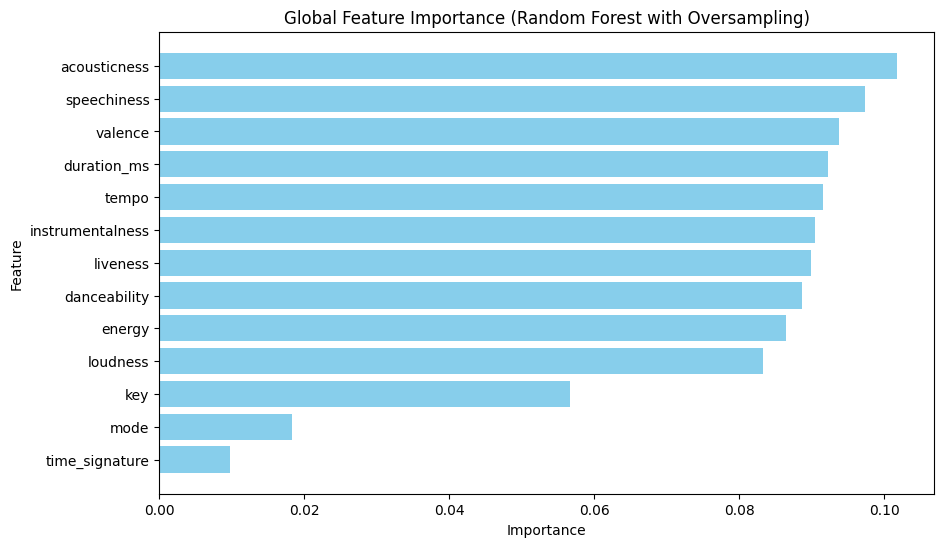
\includegraphics[width=\linewidth]{media/random_forest_feature_imp_global.png}
        \caption{Global Feature Importance Using Random Forests Model}
    \end{minipage}%
    \hspace{0.05\textwidth} % Space between the two figures
    \begin{minipage}{0.45\textwidth}
        \centering
        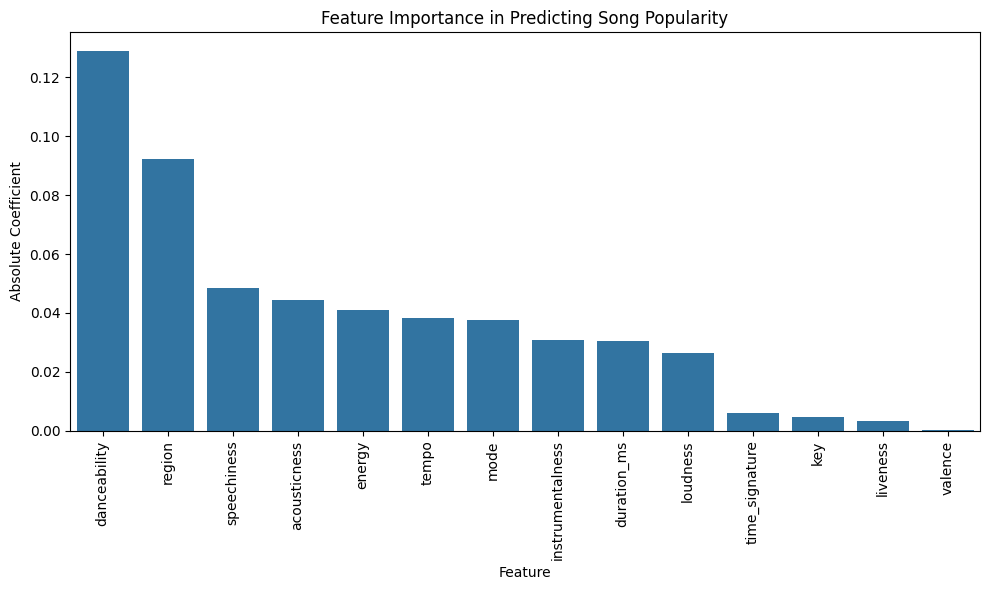
\includegraphics[width=\linewidth]{media/logistic_reg_feature_imp_global.png}
        \caption{Global Feature Importance Using Logistic Regression Model}
    \end{minipage}
\end{figure}
\begin{figure}[h]
    \centering
    \begin{minipage}{0.45\textwidth}
        \centering
        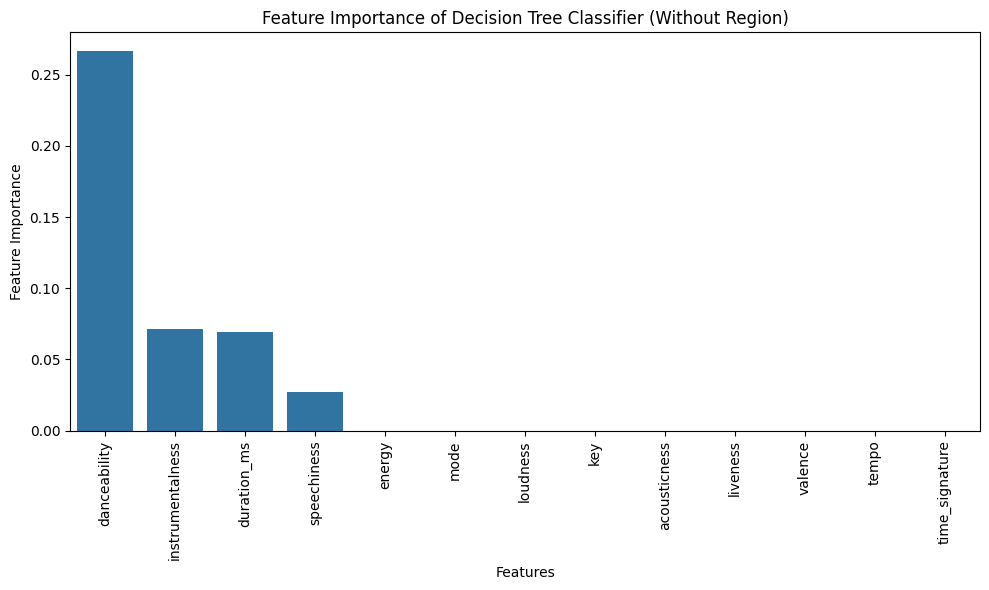
\includegraphics[width=\linewidth]{media/decision_tree_fea_imp_global.png}
        \caption{Global Feature Importance Using Decision Tree Model}
    \end{minipage}%
    \hspace{0.05\textwidth} % Space between the two figures
    \begin{minipage}{0.45\textwidth}
        \centering
        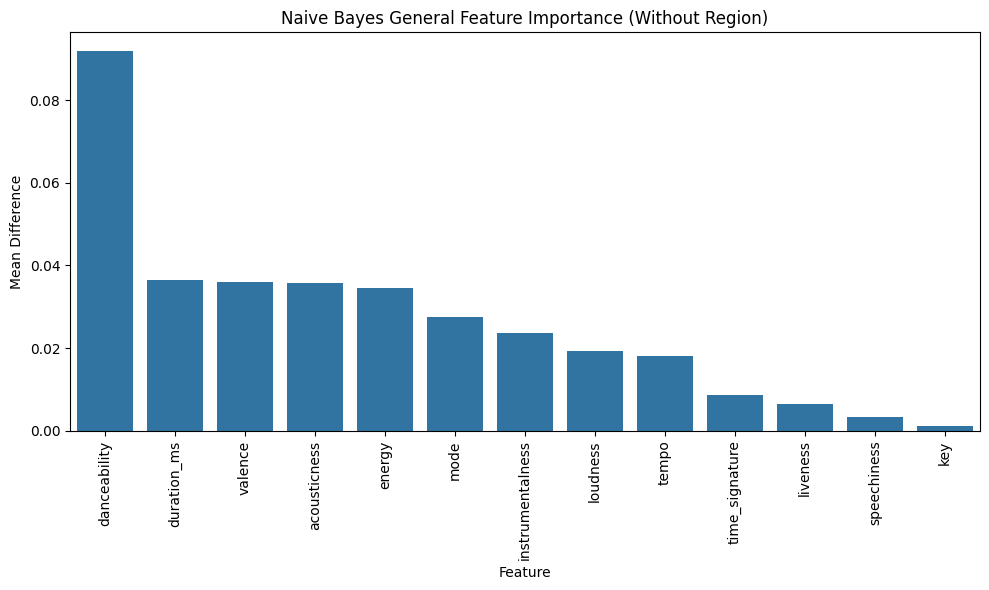
\includegraphics[width=\linewidth]{media/naive_bayes_fea_imp_global.png}
        \caption{Global Feature Importance Using Naive Bayes Model}
    \end{minipage}
\end{figure}

\newpage

\section{Regional Feature Importance Analysis}


The feature importance is extracted not only globally but also for each region. To do that we decide to consider the Random Forest model as the best model.
This analysis helps to understand how the music tastes of different regions are shaped by audio features.
The most important features for each region are shown below. The mean values of these features are also given to help understand the music tastes of each region.

\textbf{Feature Importance for Each Region Extracted From Random Forest Model:}
\begin{figure}[h]
    \centering
    \begin{minipage}{0.45\textwidth}
        \centering
        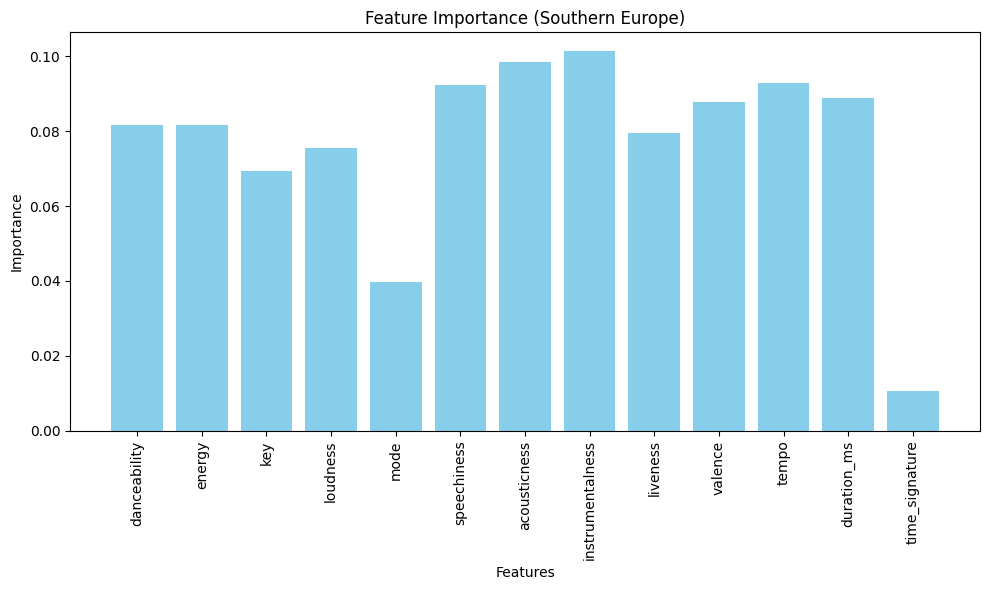
\includegraphics[width=\linewidth]{media/rf_feature_imp_northen_europe.png}
        \caption{Feature Importance in North Europe}
    \end{minipage}%
    \hspace{0.05\textwidth} % Space between the two figures
    \begin{minipage}{0.45\textwidth}
        \centering
        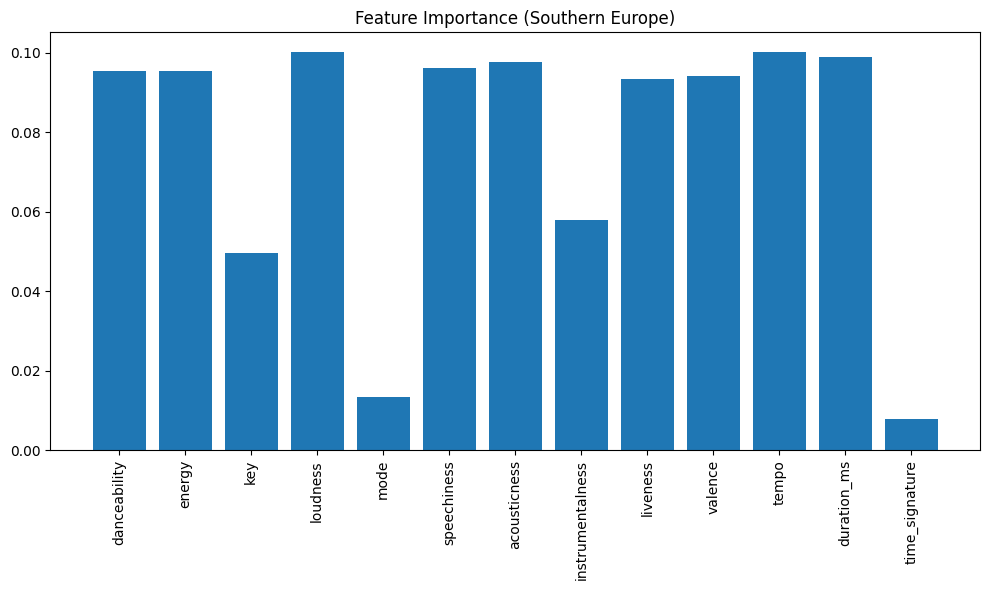
\includegraphics[width=\linewidth]{media/rf_feature_imp_southern_europe.png}
        \caption{Feature Importance in South Europe}
    \end{minipage}
\end{figure}
\begin{figure}[h]
    \centering
    \begin{minipage}{0.45\textwidth}
        \centering
        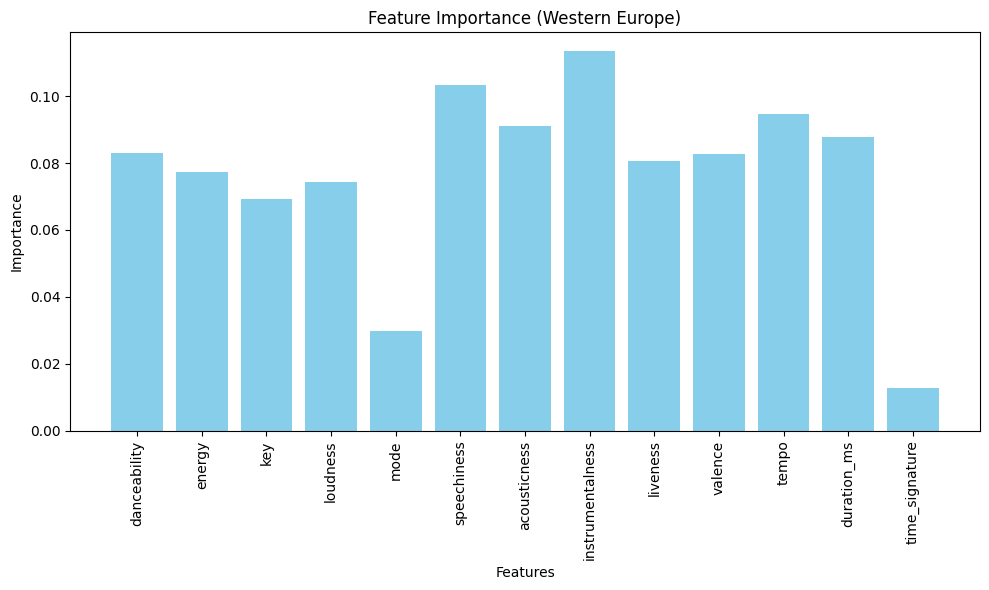
\includegraphics[width=\linewidth]{media/rf_feature_imp_western_europe.png}
        \caption{Feature Importance in Western Europe}
    \end{minipage}%
    \hspace{0.05\textwidth} % Space between the two figures
    \begin{minipage}{0.45\textwidth}
        \centering
        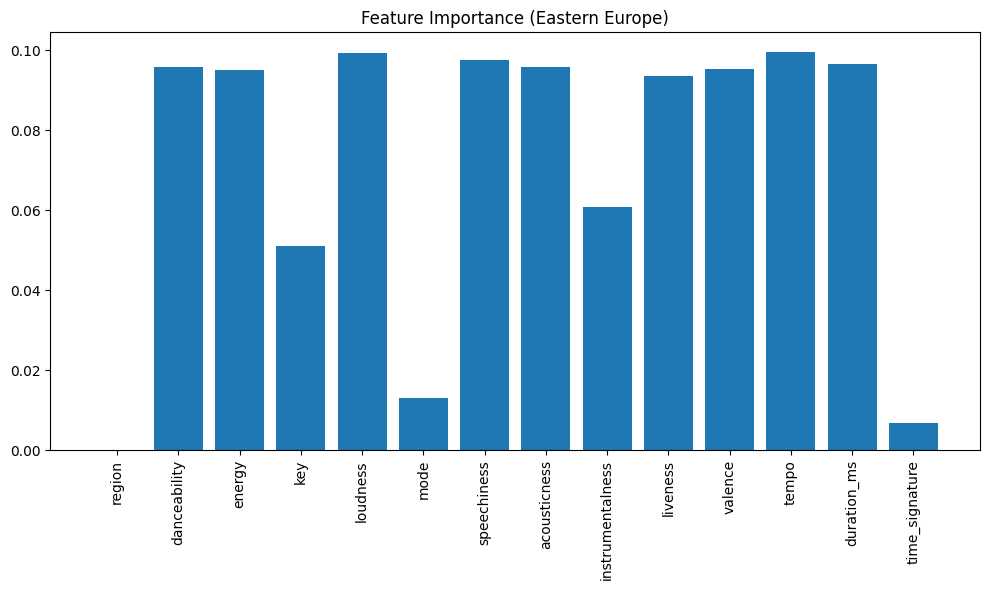
\includegraphics[width=\linewidth]{media/rf_feature_imp_eastern_europe.png}
        \caption{Feature Importance in Eastern Europe}
    \end{minipage}
\end{figure}
\begin{figure}[h]
    \centering
    \begin{minipage}{0.45\textwidth}
        \centering
        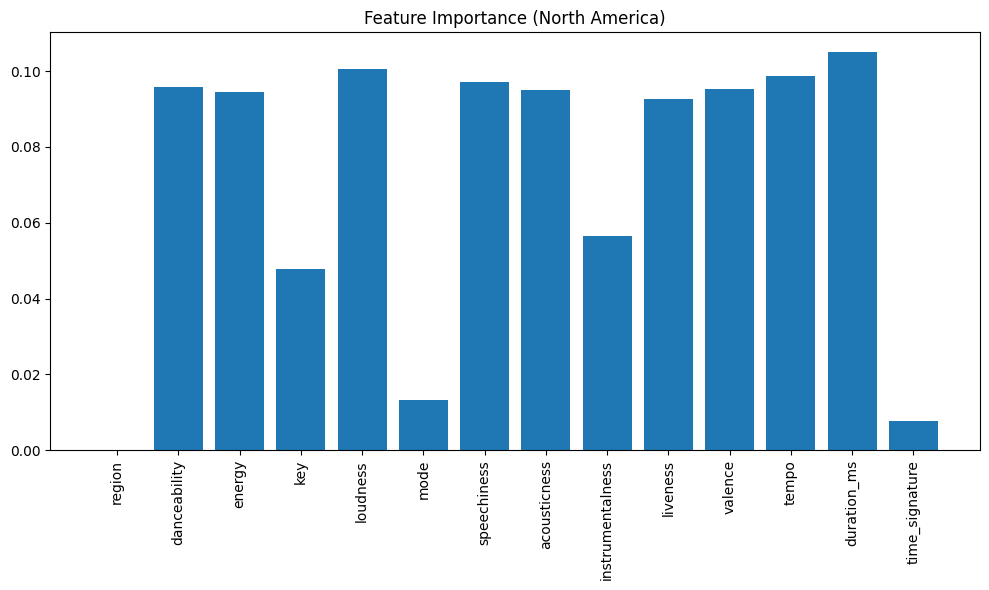
\includegraphics[width=\linewidth]{media/rf_feature_imp_north_america.png}
        \caption{Feature Importance in North America}
    \end{minipage}%
    \hspace{0.05\textwidth} % Space between the two figures
    \begin{minipage}{0.45\textwidth}
        \centering
        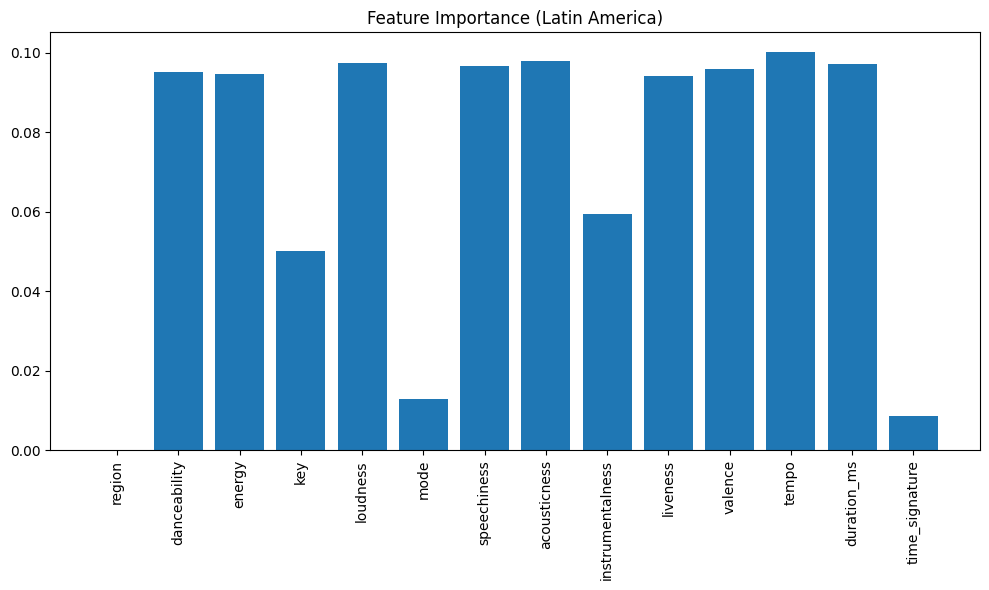
\includegraphics[width=\linewidth]{media/rf_feature_imp_latin_america.png}
        \caption{Feature Importance in Latin America}
    \end{minipage}
\end{figure}
\begin{figure}[h]
    \centering
    \begin{minipage}{0.45\textwidth}
        \centering
        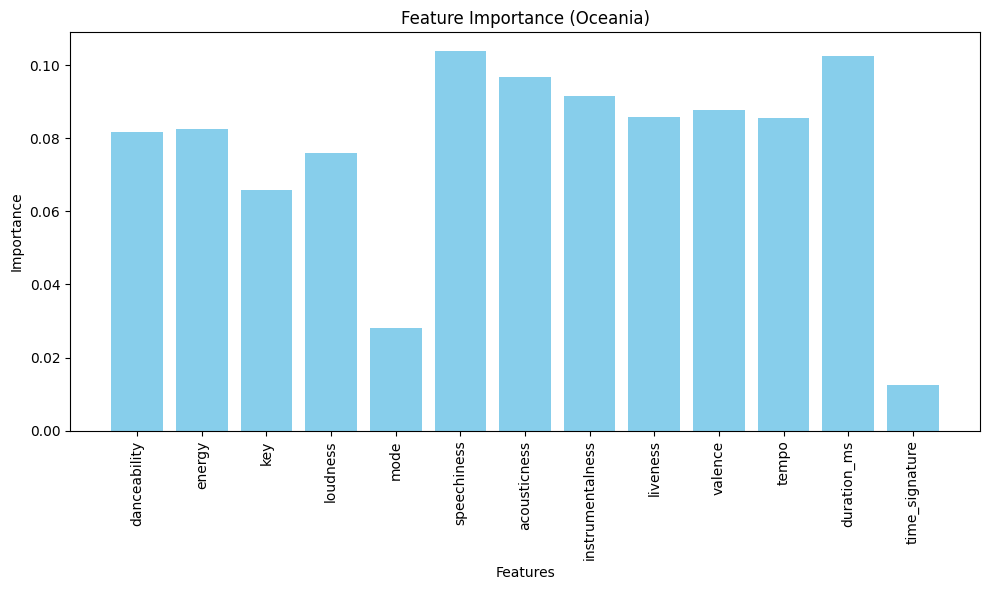
\includegraphics[width=\linewidth]{media/rf_feature_imp_ocenia.png}
        \caption{Feature Importance in Oceania}
    \end{minipage}%
    \hspace{0.05\textwidth} % Space between the two figures
    \begin{minipage}{0.45\textwidth}
        \centering
        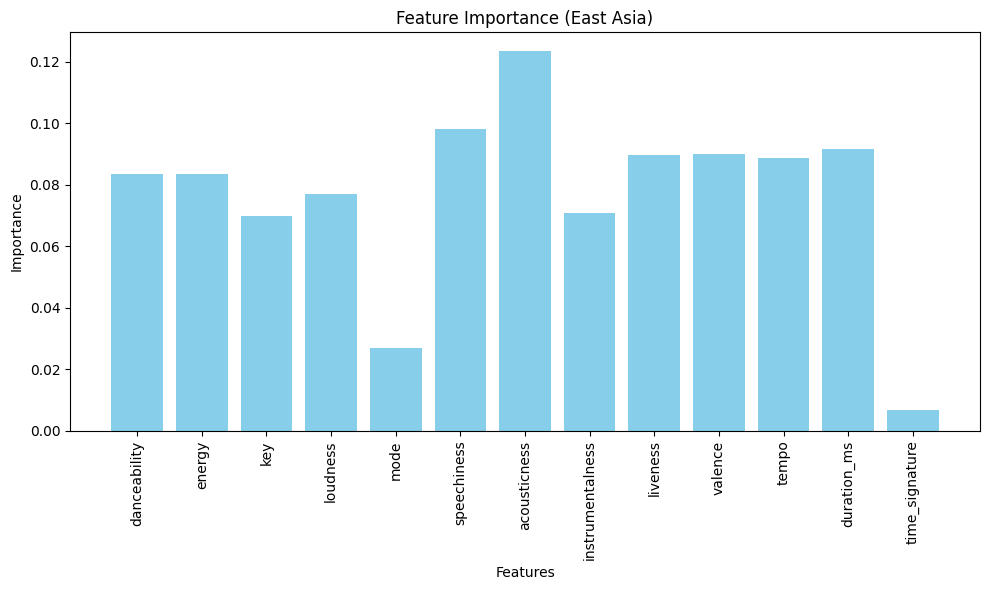
\includegraphics[width=\linewidth]{media/rf_feature_imp_east_asia.png}
        \caption{Feature Importance in East Asia}
    \end{minipage}
\end{figure}
\begin{figure}[h]
    \centering
    \begin{minipage}{0.45\textwidth}
        \centering
        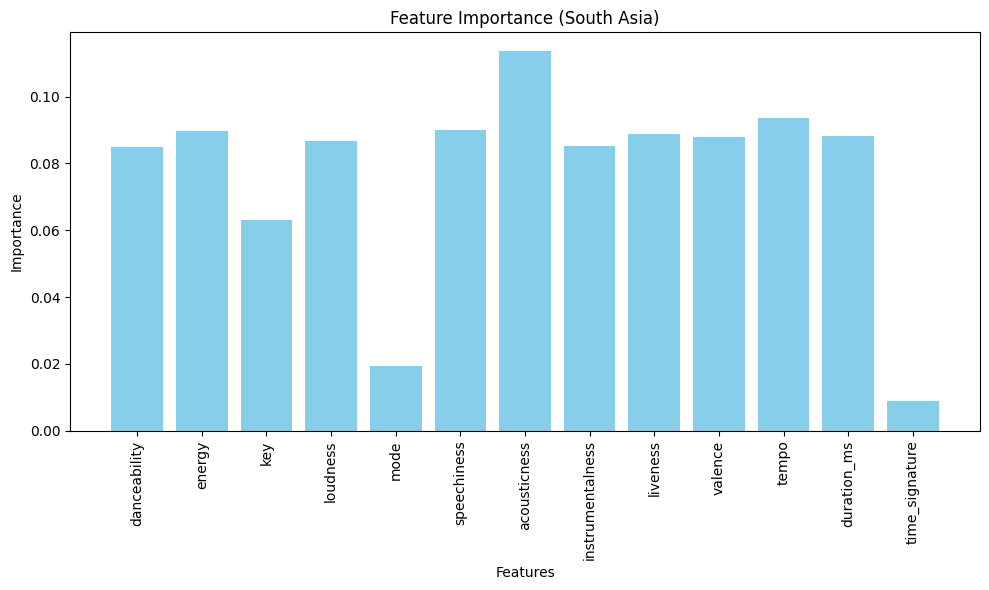
\includegraphics[width=\linewidth]{media/rf_feature_imp_south_asia.png}
        \caption{Feature Importance in South Asia}
    \end{minipage}%
    \hspace{0.05\textwidth} % Space between the two figures
    \begin{minipage}{0.45\textwidth}
        \centering
        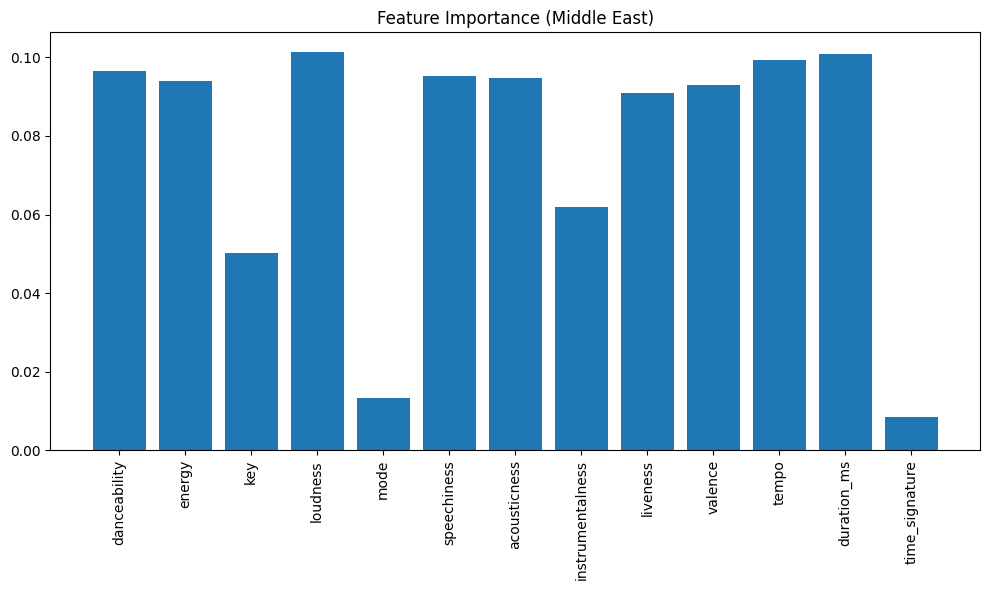
\includegraphics[width=\linewidth]{media/rf_feature_imp_middle_east.png}
        \caption{Feature Importance in Middle East}
    \end{minipage}
\end{figure}
\begin{figure}[h]
    \centering
    \begin{minipage}{0.45\textwidth}
        \centering
        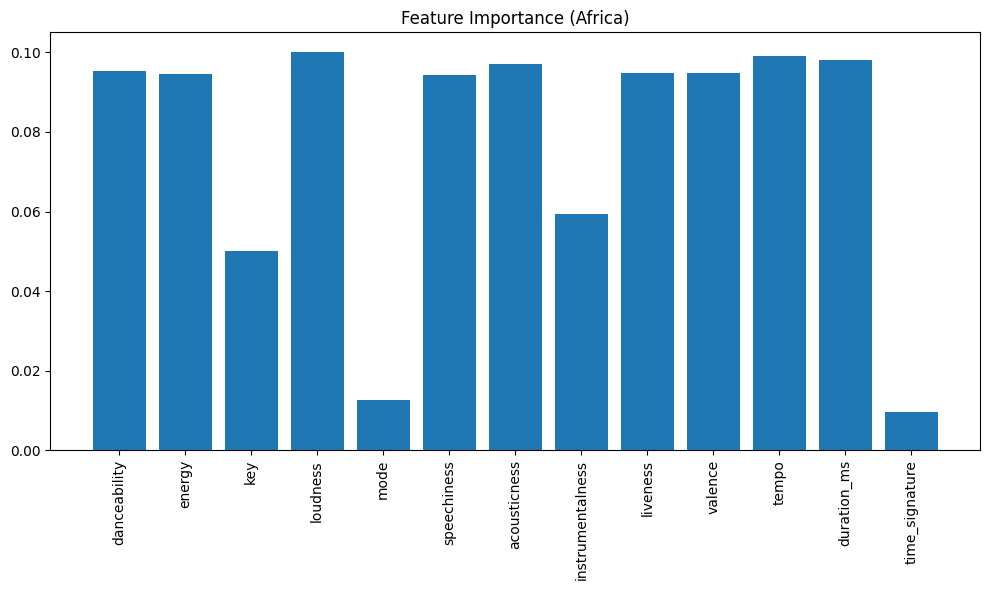
\includegraphics[width=\linewidth]{media/rf_feature_imp_africa.png}
        \caption{Feature Importance in Africa}
    \end{minipage}
\end{figure}

\clearpage 

\subsection{Important Features for Each Region and Their Mean Values:}

Generally, the different regions tend to have a coherence in the importance of the features. For example, \textit{tempo} and \textit{loudness} are among the top 5 important features in all regions. 
\textbf{Region: Northern Europe }
\begin{itemize}
    \item \textbf{Feature: duration\_ms}, Importance: 0.1021, Mean Value: 203514.75
    \item \textbf{Feature: loudness}, Importance: 0.0995, Mean Value: -7.35
    \item \textbf{Feature: tempo}, Importance: 0.0972, Mean Value: 121.29
    \item \textbf{Feature: danceability}, Importance: 0.0965, Mean Value: 0.64
    \item \textbf{Feature: acousticness}, Importance: 0.0963, Mean Value: 0.23
\end{itemize}

\textbf{Region: Southern Europe }
\begin{itemize}
    \item \textbf{Feature: loudness}, Importance: 0.1012, Mean Value: -7.02
    \item \textbf{Feature: duration\_ms}, Importance: 0.0996, Mean Value: 210862.34
    \item \textbf{Feature: tempo}, Importance: 0.0986, Mean Value: 121.24
    \item \textbf{Feature: speechiness}, Importance: 0.0968, Mean Value: 0.12
    \item \textbf{Feature: acousticness}, Importance: 0.0965, Mean Value: 0.27
\end{itemize}

\textbf{Region: Western Europe }
\begin{itemize}
    \item \textbf{Feature: loudness}, Importance: 0.1006, Mean Value: -7.26
    \item \textbf{Feature: tempo}, Importance: 0.1004, Mean Value: 120.90
    \item \textbf{Feature: duration\_ms}, Importance: 0.0990, Mean Value: 205864.40
    \item \textbf{Feature: acousticness}, Importance: 0.0965, Mean Value: 0.25
    \item \textbf{Feature: speechiness}, Importance: 0.0960, Mean Value: 0.15
\end{itemize}

\textbf{Region: Eastern Europe }
\begin{itemize}
    \item \textbf{Feature: tempo}, Importance: 0.0995, Mean Value: 122.33
    \item \textbf{Feature: loudness}, Importance: 0.0993, Mean Value: -7.34
    \item \textbf{Feature: speechiness}, Importance: 0.0975, Mean Value: 0.13
    \item \textbf{Feature: duration\_ms}, Importance: 0.0966, Mean Value: 205515.98
    \item \textbf{Feature: acousticness}, Importance: 0.0959, Mean Value: 0.24
\end{itemize}

\textbf{Region: North America }
\begin{itemize}
    \item \textbf{Feature: duration\_ms}, Importance: 0.1050, Mean Value: 206987.98
    \item \textbf{Feature: loudness}, Importance: 0.1005, Mean Value: -6.99
    \item \textbf{Feature: tempo}, Importance: 0.0988, Mean Value: 121.36
    \item \textbf{Feature: speechiness}, Importance: 0.0972, Mean Value: 0.13
    \item \textbf{Feature: danceability}, Importance: 0.0958, Mean Value: 0.66
\end{itemize}


\textbf{Region: Latin America }
\begin{itemize}
    \item \textbf{Feature: tempo}, Importance: 0.1001, Mean Value: 122.61
    \item \textbf{Feature: acousticness}, Importance: 0.0979, Mean Value: 0.29
    \item \textbf{Feature: loudness}, Importance: 0.0974, Mean Value: -6.71
    \item \textbf{Feature: duration\_ms}, Importance: 0.0972, Mean Value: 217127.50
    \item \textbf{Feature: speechiness}, Importance: 0.0965, Mean Value: 0.11
\end{itemize}

\textbf{Region: Oceania }
\begin{itemize}
    \item \textbf{Feature: duration\_ms}, Importance: 0.1061, Mean Value: 213396.98
    \item \textbf{Feature: tempo}, Importance: 0.0986, Mean Value: 120.82
    \item \textbf{Feature: danceability}, Importance: 0.0981, Mean Value: 0.65
    \item \textbf{Feature: loudness}, Importance: 0.0977, Mean Value: -7.05
    \item \textbf{Feature: acousticness}, Importance: 0.0962, Mean Value: 0.23
\end{itemize}

\textbf{Region: East Asia }
\begin{itemize}
    \item \textbf{Feature: tempo}, Importance: 0.1027, Mean Value: 121.52
    \item \textbf{Feature: duration\_ms}, Importance: 0.1005, Mean Value: 229571.73
    \item \textbf{Feature: loudness}, Importance: 0.1004, Mean Value: -6.86
    \item \textbf{Feature: acousticness}, Importance: 0.0986, Mean Value: 0.30
    \item \textbf{Feature: speechiness}, Importance: 0.0967, Mean Value: 0.08
\end{itemize}

\textbf{Region: South Asia }
\begin{itemize}
    \item \textbf{Feature: loudness}, Importance: 0.1010, Mean Value: -7.39
    \item \textbf{Feature: duration\_ms}, Importance: 0.1006, Mean Value: 222230.31
    \item \textbf{Feature: tempo}, Importance: 0.0982, Mean Value: 119.92
    \item \textbf{Feature: acousticness}, Importance: 0.0981, Mean Value: 0.36
    \item \textbf{Feature: danceability}, Importance: 0.0960, Mean Value: 0.62
\end{itemize}


\textbf{Region: Middle East }
\begin{itemize}
    \item \textbf{Feature: duration\_ms}, Importance: 0.1019, Mean Value: 213894.57
    \item \textbf{Feature: loudness}, Importance: 0.0988, Mean Value: -7.63
    \item \textbf{Feature: tempo}, Importance: 0.0976, Mean Value: 120.14
    \item \textbf{Feature: acousticness}, Importance: 0.0961, Mean Value: 0.30
    \item \textbf{Feature: danceability}, Importance: 0.0954, Mean Value: 0.64
\end{itemize}


\textbf{Region: Africa }
\begin{itemize}
    \item \textbf{Feature: loudness}, Importance: 0.0992, Mean Value: -7.61
    \item \textbf{Feature: tempo}, Importance: 0.0987, Mean Value: 120.41
    \item \textbf{Feature: duration\_ms}, Importance: 0.0976, Mean Value: 219551.52
    \item \textbf{Feature: acousticness}, Importance: 0.0963, Mean Value: 0.26
    \item \textbf{Feature: liveness}, Importance: 0.0962, Mean Value: 0.17
\end{itemize}

\subsection{Interpretation of the Results}
\begin{itemize}
    \item\textbf{Tempo Variation}
    
While tempo is among the top 5 most important features in all regions, there is a clear variation in its mean values:
The highest tempo is in Latin America (122.61), while the lowest is in South Asia (119.92).
This suggests that Latin American music tends to have a slightly faster rhythm compared to South Asian music. These differences could reflect the regions' cultural preferences for more energetic or relaxed musical styles.
\item\textbf{Loudness Preferences}

Loudness is another common feature across all regions, yet it shows notable differences in mean values:
For instance, North America (-6.99) and Latin America (-6.71) tend to prefer louder music compared to regions like Eastern Europe (-7.34) and South Asia (-7.39).
These differences could indicate varying preferences for more dynamic or intense sound production, with North and Latin America leaning toward more "in-your-face" soundscapes, while regions like Eastern Europe and South Asia favor softer or more subdued sound levels.
\item\textbf{Regional Focus on Danceability}

Danceability is present in the top 5 important features in five regions: Middle East, North America, Northern Europe, Oceania, and South Asia.
This suggests that these regions emphasize the rhythmic elements of music that facilitate dancing, perhaps reflecting a stronger cultural or social inclination towards dance-centric activities. Regions like Eastern Europe or East Asia, where danceability is not in the top 5, may prioritize other aspects of music like lyrical content or acoustic richness.
\item\textbf{Acousticness Differences}

Acousticness, which measures the likelihood of a track being acoustic, shows varying importance across regions:
South Asia has a relatively high mean acousticness (0.36), while Latin America and Oceania have lower values (0.29 and 0.23 respectively).
This could indicate a stronger preference for traditional, organic instruments in South Asia, whereas Latin America and Oceania might favor more synthesized or electronic soundscapes.
\item\textbf{Speechiness and Spoken Elements}

Speechiness is featured in several regions, but the mean values show regional differences in how much spoken word is present in music:
For instance, Latin America (0.11) and East Asia (0.08) have lower speechiness compared to Eastern Europe (0.13) and North America (0.13).
This variation may reflect differing musical traditions: regions with lower speechiness may prefer more melodic, sung vocals, while those with higher values could incorporate more rap or spoken word elements.
\item\textbf{Duration of Tracks}

The duration\_ms of tracks also varies across regions:
East Asia has the longest average duration (229571.73 ms), while Northern Europe has shorter tracks (203514.75 ms).
Longer tracks in East Asia may suggest a preference for more complex or drawn-out compositions, while shorter tracks in Northern Europe may reflect a preference for more concise and easily consumable music.
\item\textbf{Regional Absence of Energy and Valence}

Surprisingly, energy and valence (happiness or emotional positivity) are absent from the top 5 important features in all regions.
This suggests that, although energy and valence are often associated with the overall feel or mood of a track, they are not as influential in shaping regional music preferences as tempo, loudness, or other features like acousticness or danceability. It could mean that other characteristics are more decisive in defining regional music tastes.
\item\textbf{Cultural and Historical Contexts}

The preferences for certain features (like acousticness in South Asia or danceability in Oceania) could be influenced by regional cultural contexts:
South Asia's higher acousticness might reflect a deeper connection to traditional, acoustic music forms like classical or folk music.
Oceania’s preference for danceability could be tied to its strong tradition of social and communal dance, particularly in Pacific Island cultures.
\item\textbf{Impact of Globalization}

The fact that features like tempo and loudness are consistently important across all regions may indicate a certain degree of global musical homogenization due to the influence of global pop and electronic music.
However, the variation in mean values suggests that, despite global influences, regional music cultures maintain distinct preferences and characteristics.
\item\textbf{Evolution of Regional Music Preferences}

Over time, these differences in preferences might evolve as global trends influence local tastes, or as regions increasingly revert to traditional forms in response to external influences.
Monitoring how these values change over time could offer insights into the trajectory of regional music trends.
These considerations highlight the diversity in music preferences across regions, while also emphasizing certain universal elements that transcend cultural boundaries. Understanding these nuances helps map out how cultural and social factors influence regional music trends.
\end{itemize}

\chapter{Conclusion}

\subsection{Future Work}
For further developments of the project, it could be interesting to take into consideration also the sentiment analysis.
This can be done by studying the lyrics of the songs as it was done in the literature review. 
Finding out if a happy song is more keen to be popular than a sad song could be interesting.\\
Sentiment analysis could also be done on the reviews of the songs.
This could be done for example by analyzing what people write about a specific song or a specific artist by getting the tweets that contain the name of the artist or the song and then analyze the sentiment of the tweets. Also the most important music magazines could be analyzed to see if the reviews of the songs are positive or negative and how this affects the popularity of the song.\\
All this information can be used to improve the model.\\
Another interesting thing to do is to improve the User Interface of the application. The application could be improved by adding more features, like the possibility to search for a specific song and see its popularity, or the possibility to see the most popular songs of a specific artist.\\



\subsection{Conclusion}
In general, finding the most popular songs is a very difficult task. The popularity of a song is influenced by many factors and it is not easy to predict it. 
This project has shown that it is possible to predict the popularity of a song with a good accuracy, which could help a lot in the music industry, but it could be improved.\\
The algorithms used in this project are proved to be more accurate than the ones used in the state of the art. In the state of art the more accurate algorithm is the Logistic Regression, which has an accuracy of 0.52, while in this project it is the Random Forests with an accuracy of 0.85.\\
They both agreed on the fact that the most important feature is in general danceability, but as we went further in the research to find the most important features for different regions of the world it resulted that not all of them have danceability as the most important feature.\\
Furthermore, we found out that some features are similar in different regions of the world, like the energy, which is important in all the regions, while some others are different, like the key, which is important in some regions and not in others.\\
This shows that globalization has an influence on the music industry, but there are still some cultural differences that have to be taken into consideration.\\



%Add an image??



\end{document}

